% TrustEpisode AISec 2026 submission draft
% Compile with: latexmk -pdf -bibtex main.tex
\documentclass[sigconf,anonymous]{acmart}

\settopmatter{printacmref=false,printfolios=false}
\acmConference[AISec 2026]{AISec 2026 Submission Draft}{}{}
\acmYear{2026}
\renewcommand\footnotetextcopyrightpermission[1]{}
\pagestyle{plain}

\usepackage{booktabs}
\usepackage{multirow}
\usepackage{array}
\usepackage{amsmath}
\usepackage{graphicx}
\usepackage{url}
\usepackage{xcolor}
\usepackage{enumitem}
\usepackage{balance}
\usepackage{placeins}
\usepackage{microtype}
\usepackage{xspace}

\graphicspath{{figs/}}
\DeclareGraphicsExtensions{.pdf,.eps}

\setlength{\textfloatsep}{8pt plus 2pt minus 2pt}
\setlength{\floatsep}{6pt plus 2pt minus 2pt}
\setlength{\intextsep}{6pt plus 2pt minus 2pt}
\setlength{\abovecaptionskip}{4pt}
\setlength{\belowcaptionskip}{0pt}
\captionsetup{font=small}
\setlength{\emergencystretch}{2em}
\raggedbottom

\newcommand{\trustepisode}{\textsc{TrustEpisode}\xspace}
\newcommand{\tbd}{\texttt{pending}}

\begin{document}

\title{TrustEpisode: Deterministic Episode Formation and Manifest-Scoped Calibration for Partial EDR/NDR Telemetry}

\author{Anonymous Authors}
\affiliation{\institution{Anonymous Institution}}
\email{anonymous@anonymous.edu}

\begin{abstract}
Multi-step attacks appear as temporally dispersed endpoint and network observations rather than
one decisive alert. Correlation must therefore define which events form a candidate episode,
preserve deterministic revisions under late data, and distinguish an unsupported probability
from a low probability when telemetry is missing.

We present \trustepisode, a label-blind EDR/NDR pipeline with explicit ownership boundaries.
Evidence Fabric emits canonical events and independent source-health intervals; Episode
Synthesis alone owns membership and immutable revisions; a two-feature stateless scorer emits
a raw logit; and a manifest-scoped affine calibrator emits a nullable maliciousness
probability. A separate deterministic evaluator reports a five-axis evidence-sufficiency
profile without changing that probability. An AuditRecord Assembler creates one terminal,
append-only outcome per revision: a complete AuditRecord from independently produced inputs, or
an explicit AssemblyFailureRecord without fabricated score or probability fields.

We specify a frozen controlled-laboratory protocol for formation, ranking, calibration,
partial-telemetry replay, physical collector outage, and deterministic replay. The protocol
fixes candidate populations, split assignment, thresholds, group-calibration gates,
interventions, matching, metrics, resampling, and empty RT1--RT7 result schemas before locked
test access. Empirical result cells remain \texttt{pending}; no synthetic performance values
or confidence intervals are reported.
\end{abstract}

\keywords{attack episode formation, probability calibration, partial telemetry, provenance, EDR, NDR}

\maketitle
\fancyhf{}
\renewcommand{\headrulewidth}{0pt}
\fancyfoot[c]{\thepage}

\section{Introduction}
\label{sec:introduction}

Security operations and digital-forensic investigations reconstruct multi-step attacks from
temporally dispersed endpoint and network observations~\cite{alertfatigue2025,nist80086,breitinger2025sok}.
Isolated EDR or NDR records may appear benign alone yet become material when linked by time,
entity, session, and process relations. Reconstruction is not only a clustering problem:
investigators need a contract that fixes who owns episode membership, how late evidence is
admitted, how collector health differs from ``no detection,'' and how every revision leaves an
independently verifiable terminal outcome~\cite{casey2011digitalevidence,carrier2005filesystem,vanini2024timeanchors}.

Prior alert-correlation and provenance systems motivate multi-stage context using rules, graphs,
and learned representations~\cite{ning2002attackscenarios,holmes2019,unicorn2020,nodlink2024,kairos2024,captain2025}.
Those lines do not remove the need for fixed ownership of membership, immutable revision history,
and replayable audit semantics under incomplete observability. This submission evaluates
\trustepisode as a \emph{deterministic, auditable reconstruction contract} for EDR/NDR evidence.
A compact scorer and calibrator remain optional schema interfaces and are not empirically
validated here.

\paragraph{Research questions.}
\begin{enumerate}[leftmargin=*,itemsep=1pt,topsep=2pt]
  \item[\textbf{RQ1}] Under identical sealed EDR/NDR evidence, does TrustEpisode reproduce
        byte-identical membership, revision history, late-evidence records, and digests on all
        60 malicious runs?
  \item[\textbf{RQ2}] Do open, finalized, late-successor, closed, beyond-horizon, duplicate, and
        all seven AssemblyFailureRecord codes yield explicit immutable audit outcomes without
        rewriting earlier history?
  \item[\textbf{RQ3}] When a required action is absent from a reconstructed episode, can the
        pipeline localize loss across the closed A--G taxonomy, and is that taxonomy instantiated
        on sealed live evidence?
  \item[\textbf{RQ4}] Which relation, hub, merge, and late-revision mechanisms does the live
        M1--M6 cohort exercise, and which require targeted conformance cards?
  \item[\textbf{RQ5}] What portion of observed formation gain comes from replacing fixed bins
        with sliding sessionization, and does relation-aware logic provide additional measurable
        benefit on the sealed cohort?
\end{enumerate}

\paragraph{Contributions.}
\begin{enumerate}[leftmargin=*,itemsep=1pt,topsep=2pt]
  \item a single-owner immutable reconstruction contract: Episode Synthesis alone owns
        membership; late evidence yields successors or LateEvidenceRecords; deadlines do not
        extend; terminal history is append-only;
  \item replayable forensic audit outcomes with exactly one terminal AssemblyOutcome per
        revision, canonical references, SHA-256 digests, and a complete seven-code failure matrix;
  \item a stage-localized A--G evidence-loss taxonomy, conformance-tested across classes and
        instantiated on sealed M2 as \texttt{D\_token\_mapping\_failure};
  \item a fair negative-result evaluation: legacy fixed bins underperform sliding sessionization,
        while fair sliding EB1--EB4 show no observed difference on 60 sealed runs; advanced
        guards require targeted cards not mixed into primary effectiveness;
  \item a determinism boundary on all 60 sealed malicious runs: canonical ordered replay and
        duplicate retries are stable; raw delivery-order permutations are not order-robust
        without re-canonicalization; formation is single-writer per run;
  \item a contract-ablation comparison (AB0--AB3) isolating which forensic failure modes mutable,
        noncanonical, and silent-failure stores admit relative to TrustEpisode.
\end{enumerate}

\section{Related Work}
\label{sec:related}

\subsection{Alert Correlation and Attack Reconstruction}

Classical alert correlation reconstructs multi-step scenarios from intrusion alerts by temporal
and causal linking~\cite{ning2002attackscenarios}. Provenance-based detectors such as HOLMES,
UNICORN, KAIROS, NODLINK, and CAPTAIN recover APT context from system graphs and alerts
~\cite{holmes2019,unicorn2020,kairos2024,nodlink2024,captain2025}. Those systems motivate episode
construction; they do not by themselves fix single-owner membership, late-data revision policy,
or append-only terminal audit outcomes for mixed EDR/NDR streams.

\subsection{Digital Forensic Event Reconstruction}

Timeline-based event reconstruction is a core digital-forensic technique for inferring past
activity from heterogeneous artifacts~\cite{breitinger2025sok,casey2011digitalevidence}. Recent
work formalizes timestamp interpretation via time anchors and clock-skew anomalies
~\cite{vanini2024timeanchors} and surveys challenges beyond mere data volume
~\cite{breitinger2025sok}. Process models and filesystem analysis emphasize documenting what was
examined, what was unavailable, and how conclusions depend on incomplete traces
~\cite{carrier2005filesystem,nist80086}. TrustEpisode imports these audit requirements into
\emph{online} EDR/NDR episode reconstruction: immutable revisions, explicit late stores, and
digestable terminal outcomes under delayed delivery.

\subsection{Reproducibility, Tool Validation, and Provenance}

Forensic tool and method validation requires documented procedures, known datasets, and
repeatable results before casework~\cite{swgde2018tooltesting,brunty2022validation,wales2026validation}.
Chain-of-custody and provenance discipline demand that investigators show integrity of examined
objects and distinguish observed from unavailable evidence~\cite{casey2011digitalevidence,nist80086}.
TrustEpisode's contribution is not a higher detector F1; it is a single-owner revision contract,
canonical replay boundary, and explicit terminal failure semantics that make reconstruction
outcomes auditable under the same reproducibility expectations.

\subsection{Incomplete Telemetry and Evidence-Loss Attribution}

EDR and NDR fail differently; missing modality, parser blind spots, and collector health can
erase or distort attack steps without implying that correlation ``missed'' an already-normalized
event~\cite{missingmodality2024,vaseghipanah2026blindspots}. Reconstruction contracts must
therefore separate sensor observability, normalization/token mapping, formation membership, and
offline attribution when diagnosing incomplete episodes.

\subsection{Positioning Summary}

Table~\ref{tab:related-compare} contrasts representative lines along forensic-contract properties.
Unknown cells are marked \emph{Not reported}; we do not infer undocumented product behavior.
\trustepisode's novelty is the audit lifecycle and evidence-loss localization contract, not a new
graph algorithm or classifier.

\begin{table*}[!t]
\caption{Related-work comparison on forensic reconstruction contract properties (Not reported =
not documented in the cited source).}
\label{tab:related-compare}
\centering
\scriptsize
\setlength{\tabcolsep}{2.5pt}
\begin{tabular}{@{}p{0.14\textwidth}cccccccc@{}}
\toprule
\textbf{Work} & \textbf{EDR+NDR} & \textbf{Imm.\ rev.} & \textbf{Late evid.} & \textbf{Canon.\ replay} & \textbf{Term.\ fail} & \textbf{Src health} & \textbf{Loss loc.} & \textbf{Live} \\
\midrule
Alert correlation~\cite{ning2002attackscenarios} & No & Not reported & Not reported & Not reported & Not reported & Not reported & Not reported & Yes \\
HOLMES~\cite{holmes2019} & Partial & Not reported & Not reported & Not reported & Not reported & Not reported & Not reported & Yes \\
UNICORN~\cite{unicorn2020} & No & Not reported & Not reported & Not reported & Not reported & Not reported & Not reported & Yes \\
KAIROS~\cite{kairos2024} & No & Not reported & Not reported & Not reported & Not reported & Not reported & Not reported & Yes \\
Timeline SoK~\cite{breitinger2025sok} & Survey & Survey & Survey & Survey & Survey & Survey & Survey & Survey \\
Time anchors~\cite{vanini2024timeanchors} & No & Not reported & Not reported & Not reported & Not reported & Not reported & Clock skew & Yes \\
\trustepisode (this) & Yes & Yes & Yes & Yes & Yes & Yes & A--G & Yes \\
\bottomrule
\end{tabular}
\end{table*}

\subsection{Scope Distinction}

\trustepisode does not claim a new graph detector, AI ranking effectiveness, attribution beyond
observable EDR/NDR, enterprise impact estimation, or autonomous response. The evaluated
contribution is a deterministic forensic reconstruction and audit contract for sealed EDR/NDR
evidence under late arrival and incomplete observability.

\section{TrustEpisode Reconstruction Contract}
\label{sec:method}

\trustepisode converts normalized EDR/NDR events and authenticated SourceCoverage into
version-scoped forensic audit records that are deterministic over canonicalized, version-bound
inputs. Episode Synthesis alone owns membership. The lifecycle is open episode $\rightarrow$
finalized revision $\rightarrow$ immutable late successor or closed lineage $\rightarrow$
beyond-horizon LateEvidenceRecord. Each revision yields exactly one terminal AssemblyOutcome
(a canonical AuditRecord or an immutable AssemblyFailureRecord). Analysts and AI systems consume
these records but cannot redefine membership, source health, probability support, or terminal status.
Optional Feature Extractor / Scorer / Scope Resolver / Calibrator fields and sufficiency $U$ remain
design-only schema interfaces. Figure~\ref{fig:method-architecture} shows these boundaries; ground
truth is joined only offline.

\subsection{Investigation and Threat Model}
\label{sec:threat-model}

\paragraph{Assumptions.}
Raw pointers and the sealed evidence store are integrity-checkable; Health Monitor coverage
messages have authenticated sources; attackers may induce missing events, delayed delivery, and
duplicate retries; attackers cannot arbitrarily forge signed health state; runtime software may
fault; the offline evaluator is isolated from online formation.

\paragraph{Non-assumptions.}
We do \emph{not} assume complete telemetry, that collector silence equals downtime, that all
attacks are observable, that ground truth is available online, that model scores are reliable, or
that raw arrival order is fixed. Compromise of the Health Monitor identity, signing keys, or an
external writer-authorization layer is outside scope; SHA-256 digests do not authenticate producers.

\paragraph{Downstream-agent adversary.}
An AI assistant may be mistaken, prompt-injected, or compromised: it may omit evidence, misquote a
record, or recommend an unsafe action. It is outside the trusted computing base and has no
capability to write canonical evidence objects. The contract does not make its narrative true; it
makes any cited case claim checkable against an immutable revision and prevents the narrative from
silently becoming the forensic record.

\paragraph{Investigator workflow.}
Investigators import sealed EDR/NDR, form revisions, and inspect each terminal audit outcome.
They then check coverage and provenance, resolve late evidence, run the A--G waterfall for a
missing step, replay the digests, and report observed, unavailable, and unknown separately.

\subsection{Evidence and Reconstruction Model}
\label{sec:problem-formulation}

The core evaluated objects are NormalizedEvent, SourceCoverage, EpisodeRevision,
LateEvidenceRecord, AuditRecord, and AssemblyFailureRecord; optional design-only schema objects
are FeatureVector, SupportDecision, nullable $P$, and structured $U$. Offline labels never enter
online schemas. Table~\ref{tab:ownership} assigns producers and forbidden behaviors for both.

\begin{table*}[!t]
\caption{Single-owner online object contract.}
\label{tab:ownership}
\centering
\scriptsize
\begin{tabular}{p{0.17\textwidth}p{0.17\textwidth}p{0.29\textwidth}p{0.28\textwidth}}
\toprule
\textbf{Object} & \textbf{Sole producer} & \textbf{Consumers} & \textbf{Forbidden behavior} \\
\midrule
NormalizedEvent & Evidence Fabric & Episode Synthesis & label, scenario, or health fields \\
SourceCoverage & Health Monitor & Scope Resolver; Sufficiency; Assembler & infer outage from event silence \\
EpisodeRevision / LateEvidenceRecord & Episode Synthesis & Feature; Sufficiency; Assembler / late store & rewrite a prior revision; admit beyond-horizon into membership \\
FeatureVector $[D,C]$ & Feature Extractor & Stateless Scorer; Assembler & health/source mask; labels; scenario metadata \\
Nullable $P$ & Calibrator (design) & Assembler & numeric unsupported output \\
Structured $U$ & Sufficiency Evaluator & Assembler & scalarization that rewrites $P$ \\
AssemblyOutcome & AuditRecord Assembler & Append-only store; replay & both success and failure; update/delete \\
\bottomrule
\end{tabular}
\end{table*}

\begin{figure}[t]
  \centering
  \scriptsize
  \setlength{\fboxsep}{5pt}
  \begin{minipage}{\columnwidth}\centering
  \fbox{\parbox{0.91\columnwidth}{\centering
    \textbf{EDR/NDR events + authenticated source health}}}\\[2pt]
  $\downarrow$\\[2pt]
  \fbox{\parbox{0.91\columnwidth}{\centering
    \textbf{Evidence Fabric / Health Monitor}}}\\[2pt]
  $\downarrow$\\[2pt]
  \fbox{\parbox{0.91\columnwidth}{\centering
    \textbf{Episode Synthesis (sole membership owner)}}}\\[2pt]
  $\downarrow$\\[2pt]
  \fbox{\parbox{0.91\columnwidth}{\centering
    \textbf{AuditRecord Assembler $\rightarrow$ append-only store}}}\\[2pt]
  \textit{Offline only: labels, matching, evaluation.}
  \end{minipage}
  \caption{Label-blind online reconstruction and offline evaluation boundary.}
  \Description{A four-stage vertical flow from EDR and NDR events plus source health, through
  Evidence Fabric and Health Monitor, Episode Synthesis, and AuditRecord assembly to an
  append-only store; labels and evaluation remain offline.}
  \label{fig:method-architecture}
\end{figure}

\subsection{Independent Evidence Health and Observability}
\label{sec:evidence-health}

Event silence is not an outage. ``No detection'' is not ``unavailable.'' SourceCoverage carries
authenticated health, parser validity, and an observed source mask. Assemblers consume exact
coverage references; they do not infer health from empty event windows.

\subsection{Deterministic Episode Formation}
\label{sec:episode-synthesis}

Formation links events using process-causal, authenticated-session, endpoint-connection, and
specific-entity relations under a 300\,s maximum inter-event gap and 3600\,s maximum episode
span. Tie-breaks are deterministic under the frozen canonical ordering contract (relation precedence,
relation count, $\Delta t$, start time, episode ID). Hub suppression, parent merge, and exact
event-time ordering are part of the frozen policy. Canonical event-time ordering is a mandatory
preprocessing step of the production formation path rather than an optional replay repair: raw
delivery order is not robust, whereas re-canonicalized input reproduces byte-identical results.
Formation never reads labels, receipts, or scenario metadata.

\begin{figure*}[t]
  \centering
  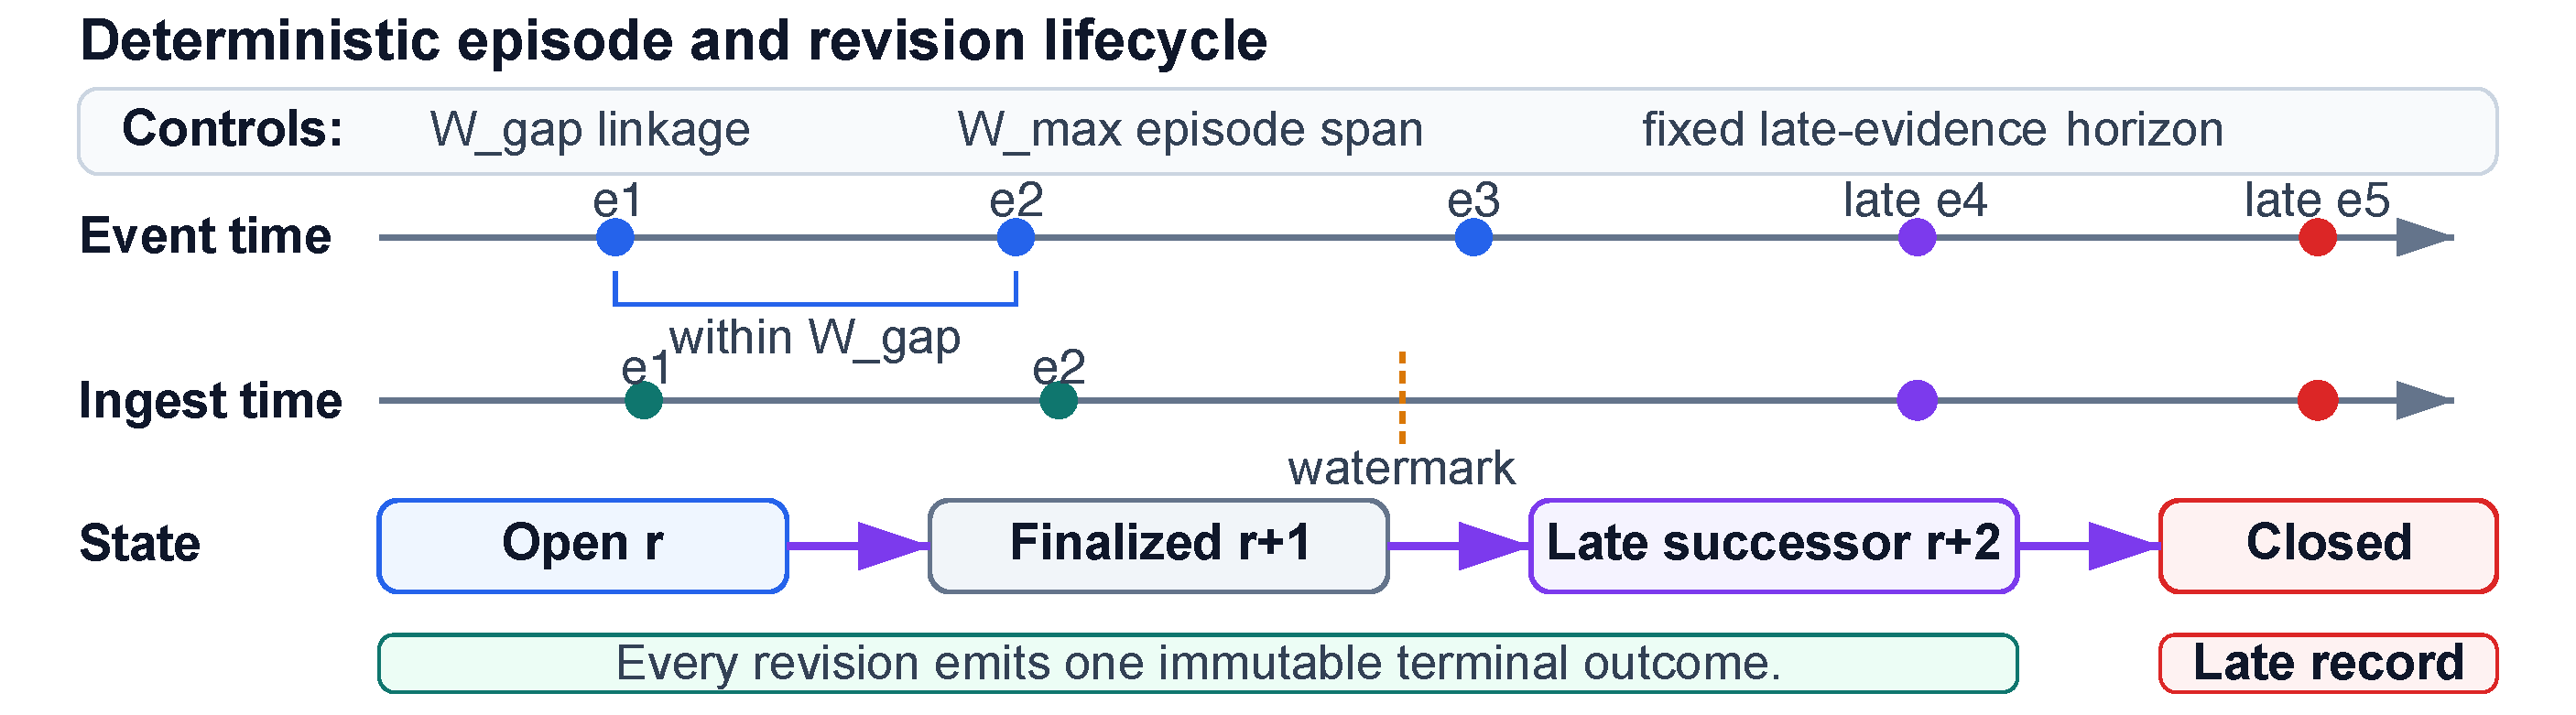
\includegraphics[width=\textwidth]{trustepisode_figures/pdf/fig02_episode_revision_lifecycle.pdf}
  \caption{Episode revision lifecycle: open $\rightarrow$ finalized $\rightarrow$ late successor or
  closed; beyond-horizon evidence enters LateEvidenceRecord without rewriting earlier membership.}
  \Description{A timeline showing event and ingest time, an open episode, finalization at a
  watermark, an immutable late-successor revision within the horizon, closure, and a separate
  late record beyond the horizon.}
  \label{fig:episode-revision-lifecycle}
\end{figure*}

\subsection{Immutable Revision Lifecycle}
\label{sec:revision-lifecycle}

A watermark lag of 120\,s advances the watermark behind observed ingest and finalizes open
episodes whose event-time end is at or before that watermark. Late evidence inside a fixed 900\,s
revision horizon may create an immutable successor; beyond-horizon or closed-lineage evidence
produces a LateEvidenceRecord. Earlier digests are never rewritten; deadlines are not extended by
late arrivals.

\subsection{Terminal Forensic Audit Contract}
\label{sec:audit-assembly}

Open episodes finalize once their event-time end is at or before the advancing watermark (lag
120\,s behind observed ingest). The assembler then applies a separate 120\,s join deadline
anchored at EpisodeRevision.watermark and inserts exactly one terminal outcome under
$(episode\_id,revision)$: AuditRecord or AssemblyFailureRecord (schema, key, duplicate, digest,
version, missing-input, timeout). These are distinct lifecycle deadlines with different anchors.
Success cannot follow terminal failure. References are canonically ordered; RFC~8785/JCS
serialization and SHA-256 digests bind versions. The store is append-only.

\subsection{Agent-Facing Evidence Boundary}
\label{sec:agent-boundary}

Downstream analyst views and AI assistants are consumers, never producers, of canonical case
facts. They receive a revision key, terminal AssemblyOutcome, ordered evidence references,
SourceCoverage references, and the independent sufficiency profile. A generated explanation or
recommended action is a noncanonical view: it cannot write EpisodeRevision, change $P$ or $U$, or
replace an AssemblyFailureRecord with success. If required inputs are missing, the only canonical
output is the failure record; an agent is not permitted to fill the gap from conversational
context. This boundary makes a later narrative falsifiable against immutable source references
without treating the language model as part of the forensic root of trust.
Section~\ref{sec:agent-boundary-conformance} tests closed-schema, support-coupling, provenance,
and digest guards. Section~\ref{sec:llm-grounding-pilot} then treats the model as an untrusted
reader and scores exact values, abstention, and pointer citations; service-identity authorization
remains a deployment assumption rather than an evaluated result.

\paragraph{Integrity is not writer authorization.}
The closed schema and unkeyed RFC~8785/SHA-256 digest validate object shape and detect an
unresealed change; they do not authenticate the producer. A downstream principal with canonical
write permission could change an allowed field and recompute the digest. The read-only boundary
therefore requires two layers: externally enforced writer authorization, plus the evaluated
schema/digest contract. AI7 is an expected-accept negative control that makes this dependency
explicit rather than treating a hash as a signature.

\subsection{Evidence-Loss Taxonomy}
\label{sec:evidence-loss-taxonomy}

When a required action token is absent from a reconstructed episode, diagnosis uses the following
closed classes (Table~\ref{tab:loss-taxonomy}):

\begin{table}[!t]
\caption{Evidence-loss taxonomy for incomplete reconstruction.}
\label{tab:loss-taxonomy}
\centering
\scriptsize
\setlength{\tabcolsep}{3pt}
\begin{tabular}{@{}>{\raggedright\arraybackslash}p{0.30\columnwidth}>{\raggedright\arraybackslash}p{0.62\columnwidth}@{}}
\toprule
\textbf{Class} & \textbf{Decision rule (summary)} \\
\midrule
\path{A_execution_failure} & Action receipt/predicate shows non-success \\
\path{B_sensor_observability_failure} & Receipt success but raw EDR/NDR lacks identifiable activity \\
\path{C_parser_or_normalization_failure} & Raw present; NormalizedEvent absent or rejected \\
\path{D_token_mapping_failure} & NormalizedEvent present under wrong/missing required token \\
\path{E_formation_membership_failure} & Correct token exists but not retained in matched episode \\
\path{F_offline_attribution_failure} & Episode retains evidence; matcher fails to credit token \\
\path{G_unknown_or_incomplete_trace} & Required supporting records missing for A--F \\
\bottomrule
\end{tabular}
\end{table}

Forbidden inference: treating episode-match F1~$=$~1.0 as exact-complete step recovery; treating
missing tokens as formation failures without a waterfall. In operational cases without a trusted
execution receipt or equivalent predicate record, the waterfall may terminate in G rather than
distinguishing execution failure from downstream evidence loss. Synthetic A--G fixtures exercise the
closed diagnostic taxonomy; they are not field validation.

\subsection{Scoring and Probability Extension (Design Only)}
\label{sec:calibration}

Design-only and unevaluated here: a Stateless Scorer consumes only $D$ and $C$ and emits
$z=f_{\theta}(D,C)$; a Scope Resolver separately consumes source availability / manifest scope and
emits a SupportDecision governing whether $P$ may be numeric. Source health must not influence $z$.
Without supported scope and a fitted version-matched calibrator, $P$ remains JSON null. Structured
$U$ cannot rewrite $z$ or $P$. This submission reports no fitted coefficients, Brier/NLL, or held-out
ranking.

\subsection{Boundary}
\label{sec:method-boundary}

The \emph{evaluated} contribution is deterministic reconstruction over canonicalized, version-bound
inputs and replayable audit semantics, including evidence-loss localization and a deployed read-only
case-materialization trace. Manifest-scoped probability is design-only. LLM generation quality, CTI
enrichment, impact scoring, autonomous response, and OT/ICS generalization are excluded.

\section{Evaluation}
\label{sec:evaluation}

The primary evaluation is an end-to-end BAS validation on isolated live Linux systems, not an
offline event-generator experiment. CALDERA executes the attack families in
Table~\ref{tab:malicious-scenarios}; \trustepisode observes only EDR/NDR telemetry and
authenticated source health. We evaluate whether the resulting episodes preserve attack
evidence and whether the five evidence-sufficiency axes in Table~\ref{tab:sufficiency} respond
faithfully under adversarial telemetry perturbations and physical collector outages. Result
cells and plots remain \tbd until the registered executions complete; no synthetic values or
confidence intervals are inserted.

\subsection{Research Questions and Evaluation Populations}
\label{sec:research-questions}

\textbf{RQ1 -- live-system validity.} Across the CALDERA scenarios in
Table~\ref{tab:malicious-scenarios}, does the label-blind builder recover the required attack
actions without excessive fragmentation, over-merge, or benign contamination?
\textbf{RQ2 -- evidence sufficiency.} Do coverage, provenance, lateness, contradiction, and
calibration states reflect the evidence actually available in each run without numerically
altering the maliciousness probability?
\textbf{RQ3 -- adversarial robustness.} Under source masking, event loss, interval removal,
delay, reordering, clock shift, duplication, and physical outage, how rapidly does performance
degrade, which faults cause explicit sufficiency transitions, and which remain silent because
authenticated health does not change?
\textbf{RQ4 -- replay and cost.} Are canonical outputs byte identical under replay, and what
throughput, latency, memory, storage, and recovery costs are observed?

The populations are disjoint views of the same registered runs. $\mathcal C_{form}$ contains
one terminal revision per surviving episode lineage at
$T_{form}=t_{run\_end}+L_{wm}+W_{rev}=t_{run\_end}+1020$ s; merged parents are removed.
$\mathcal C_{dec}^{all}$ contains the first finalized AssemblyOutcome per terminal lineage,
including supported and out-of-support AuditRecords and AssemblyFailureRecords. The scorable
inventory is
\begin{equation*}
\begin{aligned}
\mathcal C_{dec}^{score}=\{o\in\mathcal C_{dec}^{all}:&\ o\text{ is AuditRecord},\\
&o.decision\_eligible,\ P\in[0,1]\}.
\end{aligned}
\end{equation*}
After terminal insertion, the offline harness joins
$L(o)\in\{positive,negative,mixed,ambiguous\}$ by EpisodeRevision digest. Class-dependent
metrics use
\begin{equation*}
\mathcal C_{dec}^{binary}=\{o\in\mathcal C_{dec}^{score}:L(o)\in\{positive,negative\}\}.
\end{equation*}
$\mathcal C_{stream}$ retains every revision-keyed terminal outcome for sufficiency transitions,
replay equality, and cost. This separation prevents late revisions from duplicating RQ1/RQ2
candidates and prevents assembly failure from becoming hidden survivorship bias.

\subsection{CALDERA-Based Live-System Validation}
\label{sec:datasets}

The primary testbed uses CALDERA v5.3.0~\cite{caldera} as the BAS control plane, two isolated
Ubuntu 22.04 targets, and an inline Suricata gateway. Scenario commands execute against the live
process, file-system, service, and network state of the targets rather than against synthesized
logs. An instrumented endpoint wrapper records generic process start/exit observations to an
append-only spool; an independently stoppable forwarder emits label-free EDR events and
authenticated health. The inline sensor supplies NDR observations. This is a controlled
real-system validation, but it is not a production deployment or an evaluation of a commercial
EDR product.

The BAS orchestrator executes frozen no-profile Bash abilities and records action receipts in a
separate ground-truth store. CALDERA identifiers, ability metadata, receipts, and scenario labels
are excluded from the online pipeline. Every run records public software versions plus image,
configuration, parser, schema, topology, source, and hardware digests.

Table~\ref{tab:caldera-analysis-plan} specifies how the primary scenarios are analyzed. The
unchanged execution is the paired reference for each replay or outage condition. All displayed
states are placeholders until the live-system campaign completes.

\begin{table*}[t]
\caption{Planned CALDERA live-system and adversarial-robustness analysis. Each condition is
paired with the unchanged execution of the same scenario run. All result fields are pending.}
\label{tab:caldera-analysis-plan}
\centering
\scriptsize
\setlength{\tabcolsep}{3.2pt}
\begin{tabular}{p{0.15\textwidth}p{0.18\textwidth}p{0.20\textwidth}p{0.30\textwidth}p{0.08\textwidth}}
\toprule
\textbf{Analysis block} & \textbf{Paired condition} & \textbf{Primary performance readout} &
\textbf{Table~\ref{tab:sufficiency} readout} & \textbf{Status} \\
\midrule
Native BAS execution & attack-only and concurrent-benign modes & action coverage; Frag.; Merge; Contam.; episode P/R/F1 & five-axis state distribution at final revision & \tbd \\
Ranking/calibration & supported positive/negative outcomes & AUPRC; recall@10\%; Brier; NLL; eligibility rate & calibration support and provenance completeness & \tbd \\
Replay integrity stress & delay, reorder, clock shift, duplicate & paired metric change; revision count; stabilization time & lateness/provenance transitions and contradiction rate & \tbd \\
Partial telemetry & source mask, random drop, interval removal & retained action coverage; eligibility; out-of-support rate & coverage/calibration transitions and silent-loss rate & \tbd \\
Physical outage & EDR/NDR stop for 120/600 s & detection, ready, and stable-recovery times & coverage, lateness, and calibration trajectories & \tbd \\
Deterministic replay & identical input at 1/2/4/8 workers & byte equality; throughput; p50/p95/p99; peak RSS & exact equality of all five sufficiency axes & \tbd \\
\bottomrule
\end{tabular}
\end{table*}

Before a native run is sealed, the harness requires exactly one covering health interval from
both EDR instances and the NDR instance at every event-time point. Physical-outage runs omit
this gate by design so that the authenticated gap remains observable. Runs fail closed when a
manifest field is absent, a scenario action fails, or cleanup does not restore the target image.

\subsection{Ground Truth, Matching, and Labels}
\label{sec:ground-truth}

Allowlist schemas reject \path{operation_id}, \path{ability_id}, adversary/technique labels,
action receipts/windows, scenario class, and malicious labels from every online
object~\cite{kaufman2012leakage}. Each ground-truth group $g$ registers a nonempty set of required
action tokens $A_g$; each run registers benign/background tokens $B_r$. For predicted episode
$p$, $A_{cov}(p,g)=|A_p\cap A_g|/|A_g|$, where $A_p$ is its root-deduplicated attributed action
set. Offline matching constructs the threshold-qualified edge graph $E_q$. An edge requires
temporal IoU $\ge0.10$, entity Jaccard $\ge0.50$, and one exact offline receipt or registered
action. Its weight is
\begin{equation}
w=0.5A_{cov}+0.3J_{entity}+0.2\operatorname{IoU}_{time};
\quad w\ge\theta_{match}=0.50.
\label{eq:match-weight}
\end{equation}
Maximum-weight one-to-one assignment over $E_q$ operates within one run; ties use entity
overlap, absolute time difference, then ascending bytes of $(episode\_id,group\_id)$. Assignment
is used only for episode precision/recall/F1. Coverage, fragmentation, and over-merge use the
unassigned graph.

A revision chooses the first incident edge under descending $(A_{cov},w)$ then ascending group
ID. With no edge, $g^*=\texttt{null}$, $A_{cov}=0$, and $B_{cont}$ is undefined. Otherwise
\begin{equation*}
B_{cont}=\frac{|A_p\cap B_r|}{|(A_p\cap A_{g^*})\cup(A_p\cap B_r)|}.
\end{equation*}
First-match labels are mixed if $A_{cov}\ge\theta_{mal}=0.50$ and
$B_{cont}\ge\theta_{contam}=0.25$; positive if coverage passes and contamination is below the
threshold; negative if $A_{cov}=0$, a registered benign token is present, and no conflict
exists; otherwise ambiguous. Labels join only after the terminal outcome is inserted.
Sensitivity varies $\theta_{mal}\in\{.25,.50,.75\}$,
$\theta_{contam}\in\{.10,.25,.50\}$, and
$\theta_{match}\in\{.40,.50,.60\}$ without changing the primary analysis.

\begin{figure}[t]
  \centering
  \scriptsize
  \setlength{\fboxsep}{5pt}
  \begin{minipage}{\columnwidth}\centering
  \fbox{\parbox{0.91\columnwidth}{\centering
    \textbf{Online schemas reject evaluation fields}\\
    labels, receipts, windows, and scenario metadata}}\\[-1pt]
  $\downarrow$\\[-1pt]
  \fbox{\parbox{0.91\columnwidth}{\centering
    \textbf{Label-blind online pipeline}\\
    EpisodeRevision $\rightarrow$ terminal AssemblyOutcome}}\\[-1pt]
  $\downarrow$\\[-1pt]
  \fbox{\parbox{0.91\columnwidth}{\centering
    \textbf{Immutable digest join in offline harness}\\
    versioned ground truth joins only after insertion}}\\[-1pt]
  $\downarrow$\\[-1pt]
  \fbox{\parbox{0.91\columnwidth}{\centering
    \textbf{Evaluation labels and metrics}\\
    positive / negative / mixed / ambiguous}}\\[2pt]
  \textit{No evaluation field returns to inference.}
  \end{minipage}
  \caption{Ground Truth Firewall. Evaluation-only fields are rejected before inference and join
  immutable outputs only inside the offline harness.}
  \label{fig:ground-truth-firewall}
\end{figure}

\subsection{Primary BAS Scenarios}
\label{sec:scenarios}

Table~\ref{tab:malicious-scenarios} is the primary validation matrix. Each family is executed on
the live Ubuntu targets in attack-only mode and with one deterministic concurrent benign
workload. The protocol requires ten valid repetitions per family and mode; achieved counts and
all measured outcomes remain \tbd.

\begin{table*}[t]
\caption{Primary CALDERA BAS validation scenarios on live Ubuntu targets. Each card requires ten
valid repetitions in attack-only and concurrent-benign modes; achieved counts are pending.}
\label{tab:malicious-scenarios}
\centering
\scriptsize
\setlength{\tabcolsep}{3pt}
\begin{tabular}{p{0.04\textwidth}p{0.30\textwidth}p{0.17\textwidth}p{0.23\textwidth}p{0.17\textwidth}}
\toprule
\textbf{ID} & \textbf{Ordered CALDERA ability family} & \textbf{Stressor} &
\textbf{Expected EDR/NDR evidence} & \textbf{Primary sufficiency axes} \\
\midrule
M1 & discovery $\rightarrow$ peer inventory $\rightarrow$ SSH write & lateral chain & EDR lineage + NDR connection & provenance, contradiction \\
M2 & stage $\rightarrow$ archive $\rightarrow$ SCP $\rightarrow$ delayed local action & weak-to-strong & EDR file/process + NDR transfer & lateness, provenance \\
M3 & discovery $\rightarrow$ temporary-key SSH write & remote execution & EDR process + NDR session & coverage, calibration \\
M4 & five-request 60 s cadence $\rightarrow$ local action & sparse sequence & NDR cadence + EDR action & coverage, lateness \\
M5 & discovery $\rightarrow$ local configuration action & source-asymmetric case & EDR evidence; valid NDR no-detection & coverage, calibration \\
M6 & matched-tool SSH $\rightarrow$ remote write & benign-tool overlap & contextual EDR/NDR evidence & contradiction, provenance \\
M7 & actions at 0/300/3900 s & gap/span boundaries & boundary revisions and late evidence & lateness, provenance \\
\bottomrule
\end{tabular}
\end{table*}

B1--B8 cover Linux inventory, manifest-pinned package installation, file synchronization,
registered service scanning, read-only SSH administration, log collection, configuration
management, and supervisor-backed maintenance. Each benign card is run alone and as the
registered concurrent background for malicious cards. Every card fixes preconditions, exact
command templates, monotonic start offsets, fixed target paths, offline-only receipts,
postconditions, cleanup, and failure predicates. Collection or action failure remains in the
failure log but is excluded from performance estimates; cleanup failure blocks image reuse.

\subsection{Adversarial Perturbations and Physical Outage}
\label{sec:partial-telemetry}

Each valid Table~\ref{tab:malicious-scenarios} execution has an immutable unchanged replay and
deterministic adversarial children. Conditions are source masking; EDR- or NDR-specific random
drop at 5/10/25\%; removal of a 30/120/300 s interval; ingest delay of 30/120/600 s; reordering
inside 30/120/600 s buffers; event-time shifts of $-120/-30/+30/+120$ s; and duplicate root
groups at 5/10/25\%. Other-source events and the original SourceCoverage journal remain fixed,
so replay isolates data-integrity stress from health-reporting stress.

The perturbation seed is domain-separated by base run, operator, source, and dose. Before the
operator is applied, base events sort by
\begin{equation*}
(t^{event},t^{ingest},source\_instance,event\_id).
\end{equation*}
Duplicate IDs are derived from the sealed seed and original event ID; collisions invalidate the
child. These rules make every adversarial condition exactly replayable without selecting an
outcome after observing labels.

Physical outage is evaluated separately because it changes authenticated source health rather
than only event delivery. The cohort crosses source $\in\{\mathrm{EDR},\mathrm{NDR}\}$,
duration $\in\{120,600\}$ s, and ten repetitions, balanced over M1/M3/M4/M7. After two healthy
heartbeats, the selected collector is stopped and at least one scenario ability executes during
the outage. We record health detection, first parser-valid ready interval after restoration, and
the first time followed by 900 s without another revision. Detection and recovery are
right-censored when their registered observation windows expire.

For run $r$, condition $q$, and scalar metric $m$, the paired effect is
\begin{equation}
\Delta m_{r,q}=m(r,q)-m(r,0),
\label{eq:paired-robustness}
\end{equation}
where $q=0$ is the unchanged replay. For sufficiency axis $k$ with categorical states
$a,b$, the transition matrix is
\begin{equation}
T_{k,q}(a,b)=\frac{1}{N_q}\sum_{r=1}^{N_q}
\mathbf{1}[U_k(r,0)=a\land U_k(r,q)=b].
\label{eq:sufficiency-transition}
\end{equation}
For the action-coverage metric, the silent-loss rate is
\begin{equation}
SL_q=\frac{1}{N_q}\sum_{r=1}^{N_q}\mathbf{1}
[A_{cov}(r,q)<A_{cov}(r,0)\land U(r,q)=U(r,0)].
\label{eq:silent-loss}
\end{equation}
Robustness is therefore not defined as score invariance alone. Event loss with an unchanged
authenticated health journal may leave $u_{coverage}$ unchanged by construction; the analysis
reports such cases through Equation~\ref{eq:silent-loss} rather than assigning an unsupported sufficiency
transition. A desirable response can otherwise be
stable episode evidence at low dose, graceful metric degradation at higher dose, or explicit
movement to \texttt{degraded}, \texttt{unavailable}, or \texttt{out\_of\_support} when the
probability is no longer justified. Silent confidence under missing evidence is treated as a
failure.

\begin{figure*}[t]
  \centering
  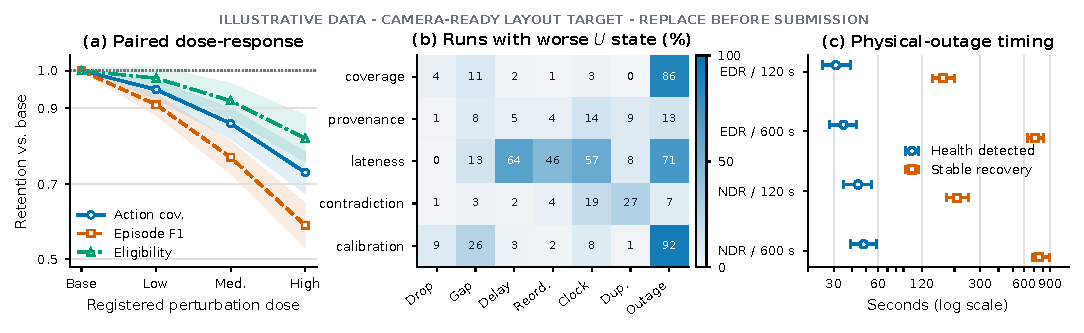
\includegraphics[width=\textwidth]{trustepisode_figures/pdf/fig10_adversarial_robustness_template.pdf}
  \caption{Illustrative camera-ready layout using simulated values, not experimental results.
  Panel (a) uses paired dose-response lines with 95\% intervals; panel (b) uses a heatmap for the
  fraction of runs moving to a worse Table~\ref{tab:sufficiency} state; panel (c) uses log-scale
  dot-and-whisker summaries for outage detection and stable recovery. All values must be replaced
  by registered measurements before submission; censored time-to-event curves belong in the
  supplementary material when censoring is material.}
  \label{fig:telemetry-perturbation-design}
\end{figure*}

\subsection{Metrics and Statistical Reporting}
\label{sec:metrics}

For run $r$, let $E_{q,r}$ be its unassigned threshold-qualified graph. For each truth group
$g$, $n_g=|\{p:(p,g)\in E_{q,r}\}|$; for episode $p$,
$d_p=|\{g:(p,g)\in E_{q,r}\}|$. Formation reporting uses run-macro action coverage,
$|G_r|^{-1}\sum_g\max(0,n_g-1)$ fragmentation,
$|P_r|^{-1}\sum_p\mathbf{1}[d_p>1]$ over-merge, mean defined contamination, and one-to-one
episode precision/recall/F1. Empty denominators are undefined, never zero.

Ranking and calibration use $\mathcal C_{dec}^{binary}$ only. AUPRC and recall among the top
$\max(1,\lceil0.10|\mathcal C_{dec,r}^{binary}|\rceil)$ per run are primary ranking metrics;
Brier, NLL, and ten-bin reliability are reported only for supported records. AUROC and
precision@$k$ are secondary~\cite{saito2015pr}. For each Table~\ref{tab:sufficiency} axis we
report state counts and proportions, the transition matrix in
Equation~\ref{eq:sufficiency-transition}, decision-eligible coverage, revision count, and time
to stable closure. Equation~\ref{eq:silent-loss} reports coverage loss not accompanied by any
sufficiency transition. Outage plots report detection, ready, and stable-recovery time with
censoring.

All summaries are macro-averaged over complete scenario runs. Paired perturbation effects use
Equation~\ref{eq:paired-robustness}; intervals use 2,000 percentile bootstrap resamples of
complete run pairs with fixed seed 20260710~\cite{field2007bootstrap}. The paper will report the
number of valid, failed, undefined, and censored runs beside every estimate. Deterministic-replay
cost is measured at 1/2/4/8 workers using one warm-up and five measured repeats, with byte
equality, throughput, ingest-to-outcome p50/p95/p99 latency, peak RSS, canonical storage bytes,
and replay time.

\subsection{External Entity-Level Context}
\label{sec:public-comparators}

Table~\ref{tab:entity-public-comparison} is secondary context, not the primary validation. It
combines entity counts reported by CAPTAIN for KAIROS, NODLINK, and CAPTAIN on DARPA TC E3
CADETS/THEIA~\cite{captain2025,kairos2024,nodlink2024} with a deterministic \trustepisode
projection. The external rows were not reproduced in this work, and the \trustepisode rows are
an entity projection from episode membership rather than a native entity classifier. HOLMES is
omitted because its reported grain is graph/campaign-level rather than an aligned E3
entity-count row~\cite{holmes2019,nodlink2024}. No cross-grain superiority claim follows.

\begin{table*}[t]
\caption{Entity-level DARPA TC E3 context. KAIROS, NODLINK, and CAPTAIN counts are transcribed
from CAPTAIN Table V~\cite{captain2025} and were not reproduced in this work. \trustepisode is
measured in this work using a deterministic projection from immutable episode membership.
Precision, recall, and F1 are derived from the displayed counts. Bold denotes the highest
precision, recall, or F1 within each dataset; ties are retained.}
\label{tab:entity-public-comparison}
\centering
\scriptsize
\setlength{\tabcolsep}{4pt}
\begin{tabular}{llrrrrrrl}
\toprule
\textbf{Dataset} & \textbf{Method} & \textbf{TP} & \textbf{FP$_{0}$} & \textbf{FN} &
\textbf{Precision} & \textbf{Recall} & \textbf{F1} & \textbf{Source} \\
\midrule
E3-CADETS & KAIROS & 15 & 1,017 & 11 & 0.015 & 0.577 & 0.028 & CAPTAIN Tbl.~V \\
 & NODLINK & 3 & 120 & 2 & 0.024 & 0.600 & 0.047 & CAPTAIN Tbl.~V \\
 & CAPTAIN & 16 & 34 & 10 & \textbf{0.320} & \textbf{0.615} & \textbf{0.421} & CAPTAIN Tbl.~V \\
 & \trustepisode & 16 & 64 & 10 & 0.200 & \textbf{0.615} & 0.302 & this work \\
\midrule
E3-THEIA & KAIROS & 12 & 3,566 & 3 & 0.003 & 0.800 & 0.007 & CAPTAIN Tbl.~V \\
 & NODLINK & 14 & 62 & 0 & 0.184 & \textbf{1.000} & 0.311 & CAPTAIN Tbl.~V \\
 & CAPTAIN & 11 & 194 & 4 & 0.054 & 0.733 & 0.100 & CAPTAIN Tbl.~V \\
 & \trustepisode & 10 & 9 & 5 & \textbf{0.526} & 0.667 & \textbf{0.588} & this work \\
\bottomrule
\end{tabular}
\end{table*}

For the reserved projection, an entity is predicted iff its canonical identifier belongs to a
decision-eligible positive terminal episode; duplicates count once per evaluation cohort. A
process-only scope aligns NODLINK, while an all-evaluable scope admits only entities in the
frozen KAIROS/CAPTAIN-aligned mapping. Projection changes no formation, score, calibration, or
threshold.

\subsection{Pending Evidence and Limitations}
\label{sec:results}
\label{sec:discussion}

The paper-facing CALDERA table and robustness figure intentionally retain \tbd markers until all
scenario repetitions, perturbation pairs, and outage traces pass validation. Replacement values
must include run counts, undefined/censored counts, and confidence intervals; a point estimate
alone is insufficient. The controlled environment demonstrates execution against live operating
systems and real EDR/NDR collection paths, but cannot establish production generalization,
unseen-evasion robustness, or field base rates. Calibration claims apply only to exact supported
manifests. The study excludes CTI, agentic response, impact/priority, OT/ICS, and autonomous
remediation.

\ifdefined\fullappendix
\clearpage
\fi
\section{Conclusion}
\label{sec:conclusion}

\trustepisode provides a deterministic, auditable EDR/NDR episode-reconstruction contract:
single-owner immutable revisions, append-only terminal outcomes with a complete failure-code
matrix, and stage-localized A--G evidence-loss diagnosis. On the sealed M1--M6 cohort, sliding
sessionization improves completeness relative to fixed bins, but fair sliding time/entity/relation
builders show \emph{no observed difference} from full TrustEpisode (60/60 ties). That negative
result is forensic evidence about benchmark coverage: advanced guards require targeted
conformance cards, which we provide without treating them as live effectiveness. Canonical
replay is byte-identical on all 60 sealed malicious runs; raw arrival-order robustness requires
re-canonicalization. M2's missing \texttt{file\_transfer} token is
\texttt{D\_token\_mapping\_failure}, not a demonstrated formation drop. Contract ablation shows
which properties prevent mutable history, silent missing-input failure, and noncanonical replay.
Supplemental partition artifacts (not primary estimators) include L1 live bases with offline
L1/L2 ablations, L3 controlled hub inject, L4 controlled late inject, wall-clock within-horizon
holds (2/2), and sealed beyond-horizon attempts without organic LateEvidenceRecord. Sealed M7 is
a supplemental 3900\,s boundary-stress cohort only. Fitted scoring, calibration, and
telemetry-outage robustness remain unevaluated and outside these claims.

\ifdefined\fullappendix
\appendix

\section{Online Data Contracts and Ownership}
\label{app:data-contracts}

\subsection{Canonical Online Schemas}

All online objects are versioned, immutable after emission, and validated against an allowlist
before storage. Table~\ref{tab:appendix-schemas} defines the minimum contract. Optional fields
may be absent but cannot change the meaning of a required field.

\begin{table*}[t]
\caption{Canonical online schema registry.}
\label{tab:appendix-schemas}
\centering
\scriptsize
\begin{tabular}{p{0.15\textwidth}p{0.17\textwidth}p{0.42\textwidth}p{0.17\textwidth}}
\toprule
\textbf{Object} & \textbf{Key} & \textbf{Required content} & \textbf{Permitted optional content} \\
\midrule
NormalizedEvent & \texttt{event\_id} & UTC event/ingest times; source family/instance; canonical subject, object, action; raw pointer; dependency group; schema/parser versions & source-native attributes on an explicit allowlist \\
SourceCoverage & source instance plus interval start & interval end; expected flag; health enum; observed lag; reason code; monitor/policy versions & authenticated diagnostic reference \\
EpisodeRevision & episode ID plus revision number & ordered events/links; lineage; state; fixed first-finalized time/deadline; watermark; policy version; membership digest & accepted-late reason and predecessor \\
LateEvidenceRecord & episode ID plus latest revision & beyond-horizon event/pointer; arrival/deadline; dependency root; reason; digest & none \\
FeatureVector & episode ID plus revision number & $D,C,m,o^{det}$; feature version; normalizer hashes; ordered input references & none \\
SupportDecision & episode ID plus revision number & resolved $a^{det}$; $\kappa$; group key; eligibility; manifest digest; coverage references & none \\
AuditRecord / AssemblyFailureRecord & episode ID plus revision number & complete joined outputs / terminal failure code and observed inputs; canonical digest & non-canonical runtime envelope \\
\bottomrule
\end{tabular}
\end{table*}

NormalizedEvent is produced only by Evidence Fabric; SourceCoverage only by Health Monitor;
EpisodeRevision and LateEvidenceRecord only by Episode Synthesis; FeatureVector only by Feature
Extractor; $z$ only by Stateless Scorer; SupportDecision only by Scope Resolver; $P$ only by
Calibrator; $U$ only by Sufficiency Evaluator; and AssemblyOutcome only by AuditRecord Assembler.
The store is only a sink:
it grants \texttt{INSERT} and \texttt{SELECT} but denies \texttt{UPDATE} and \texttt{DELETE} for every
emitted revision and record. A correction is represented by a new revision and record that
references its predecessor.

\subsection{Types, Time, Pointers, and Enums}

Identifiers are non-empty UTF-8 strings scoped by their producer version. Event and ingest
times are UTC RFC~3339 timestamps with microsecond precision. Raw pointers contain an
immutable object identifier, content digest, byte range or record locator, and storage schema
version; they never embed mutable file paths as identity. Health is one of
\{\path{healthy}, \path{degraded}, \path{down}, \path{unknown},
\path{not_applicable}\}. Every evidence reference includes its root dependency group so
that forwarded or derived copies remain one observation.

\subsection{Canonical Serialization and Digest}
\label{app:canonical-serialization}

The deterministic payload uses UTF-8 RFC 8785 JSON Canonicalization Scheme bytes, including
lexicographically ordered object keys and shortest round-trip decimal encodings. Arrays use
the schema's explicit domain order. NaN and infinities are forbidden. When
$\kappa=\kappa_\varnothing$, the
serialized probability field is the JSON literal \texttt{null}; it is never omitted, zeroed,
or replaced by an estimate. The canonical digest is SHA-256 over these bytes. Wall-clock
execution time, host name, process ID, memory address, and machine-specific runtime counters
are stored as a separate non-canonical envelope and cannot affect the digest.

The supplied schema sets \path{additionalProperties} to false for every object. It lists all
required and nested types, fixes enum values, and requires \path{decision_eligible}. It is
versioned as
\path{trustepisode_online.v1.schema.json}. The AuditRecord digest include set is every required field except
\texttt{canonical\_digest}; the runtime envelope is also excluded. Included examples validate a
supported record and a null-probability unsupported record. A third example containing
\texttt{malicious\_label} is required to fail schema validation.

\subsection{Firewall Examples}

A valid minimal record contains only online-observable fields:
\begin{quote}\small\ttfamily
event\_id=edr:0042;\\
event\_time=2026-07-10T04:00:00.000000Z;\\
ingest\_time=2026-07-10T04:00:01.120000Z;\\
source=EDR; subject=proc:p7; object=file:f9;\\
action=write; raw\_ref=sha256:...;\\
dependency\_group=root:0042; parser\_version=p3.
\end{quote}
The firewall must reject the same record if it includes, for example,
\path{ability_id=T1059-001} or \path{malicious_label=1}. Rejection fails the run-level
schema test, records the offending producer, and prevents the object from entering Episode
Synthesis. Merely ignoring a forbidden field downstream is insufficient.

\section{Episode Synthesis and Revision Algorithm}
\label{app:episode-algorithm}

\begin{figure*}[t]
  \centering
  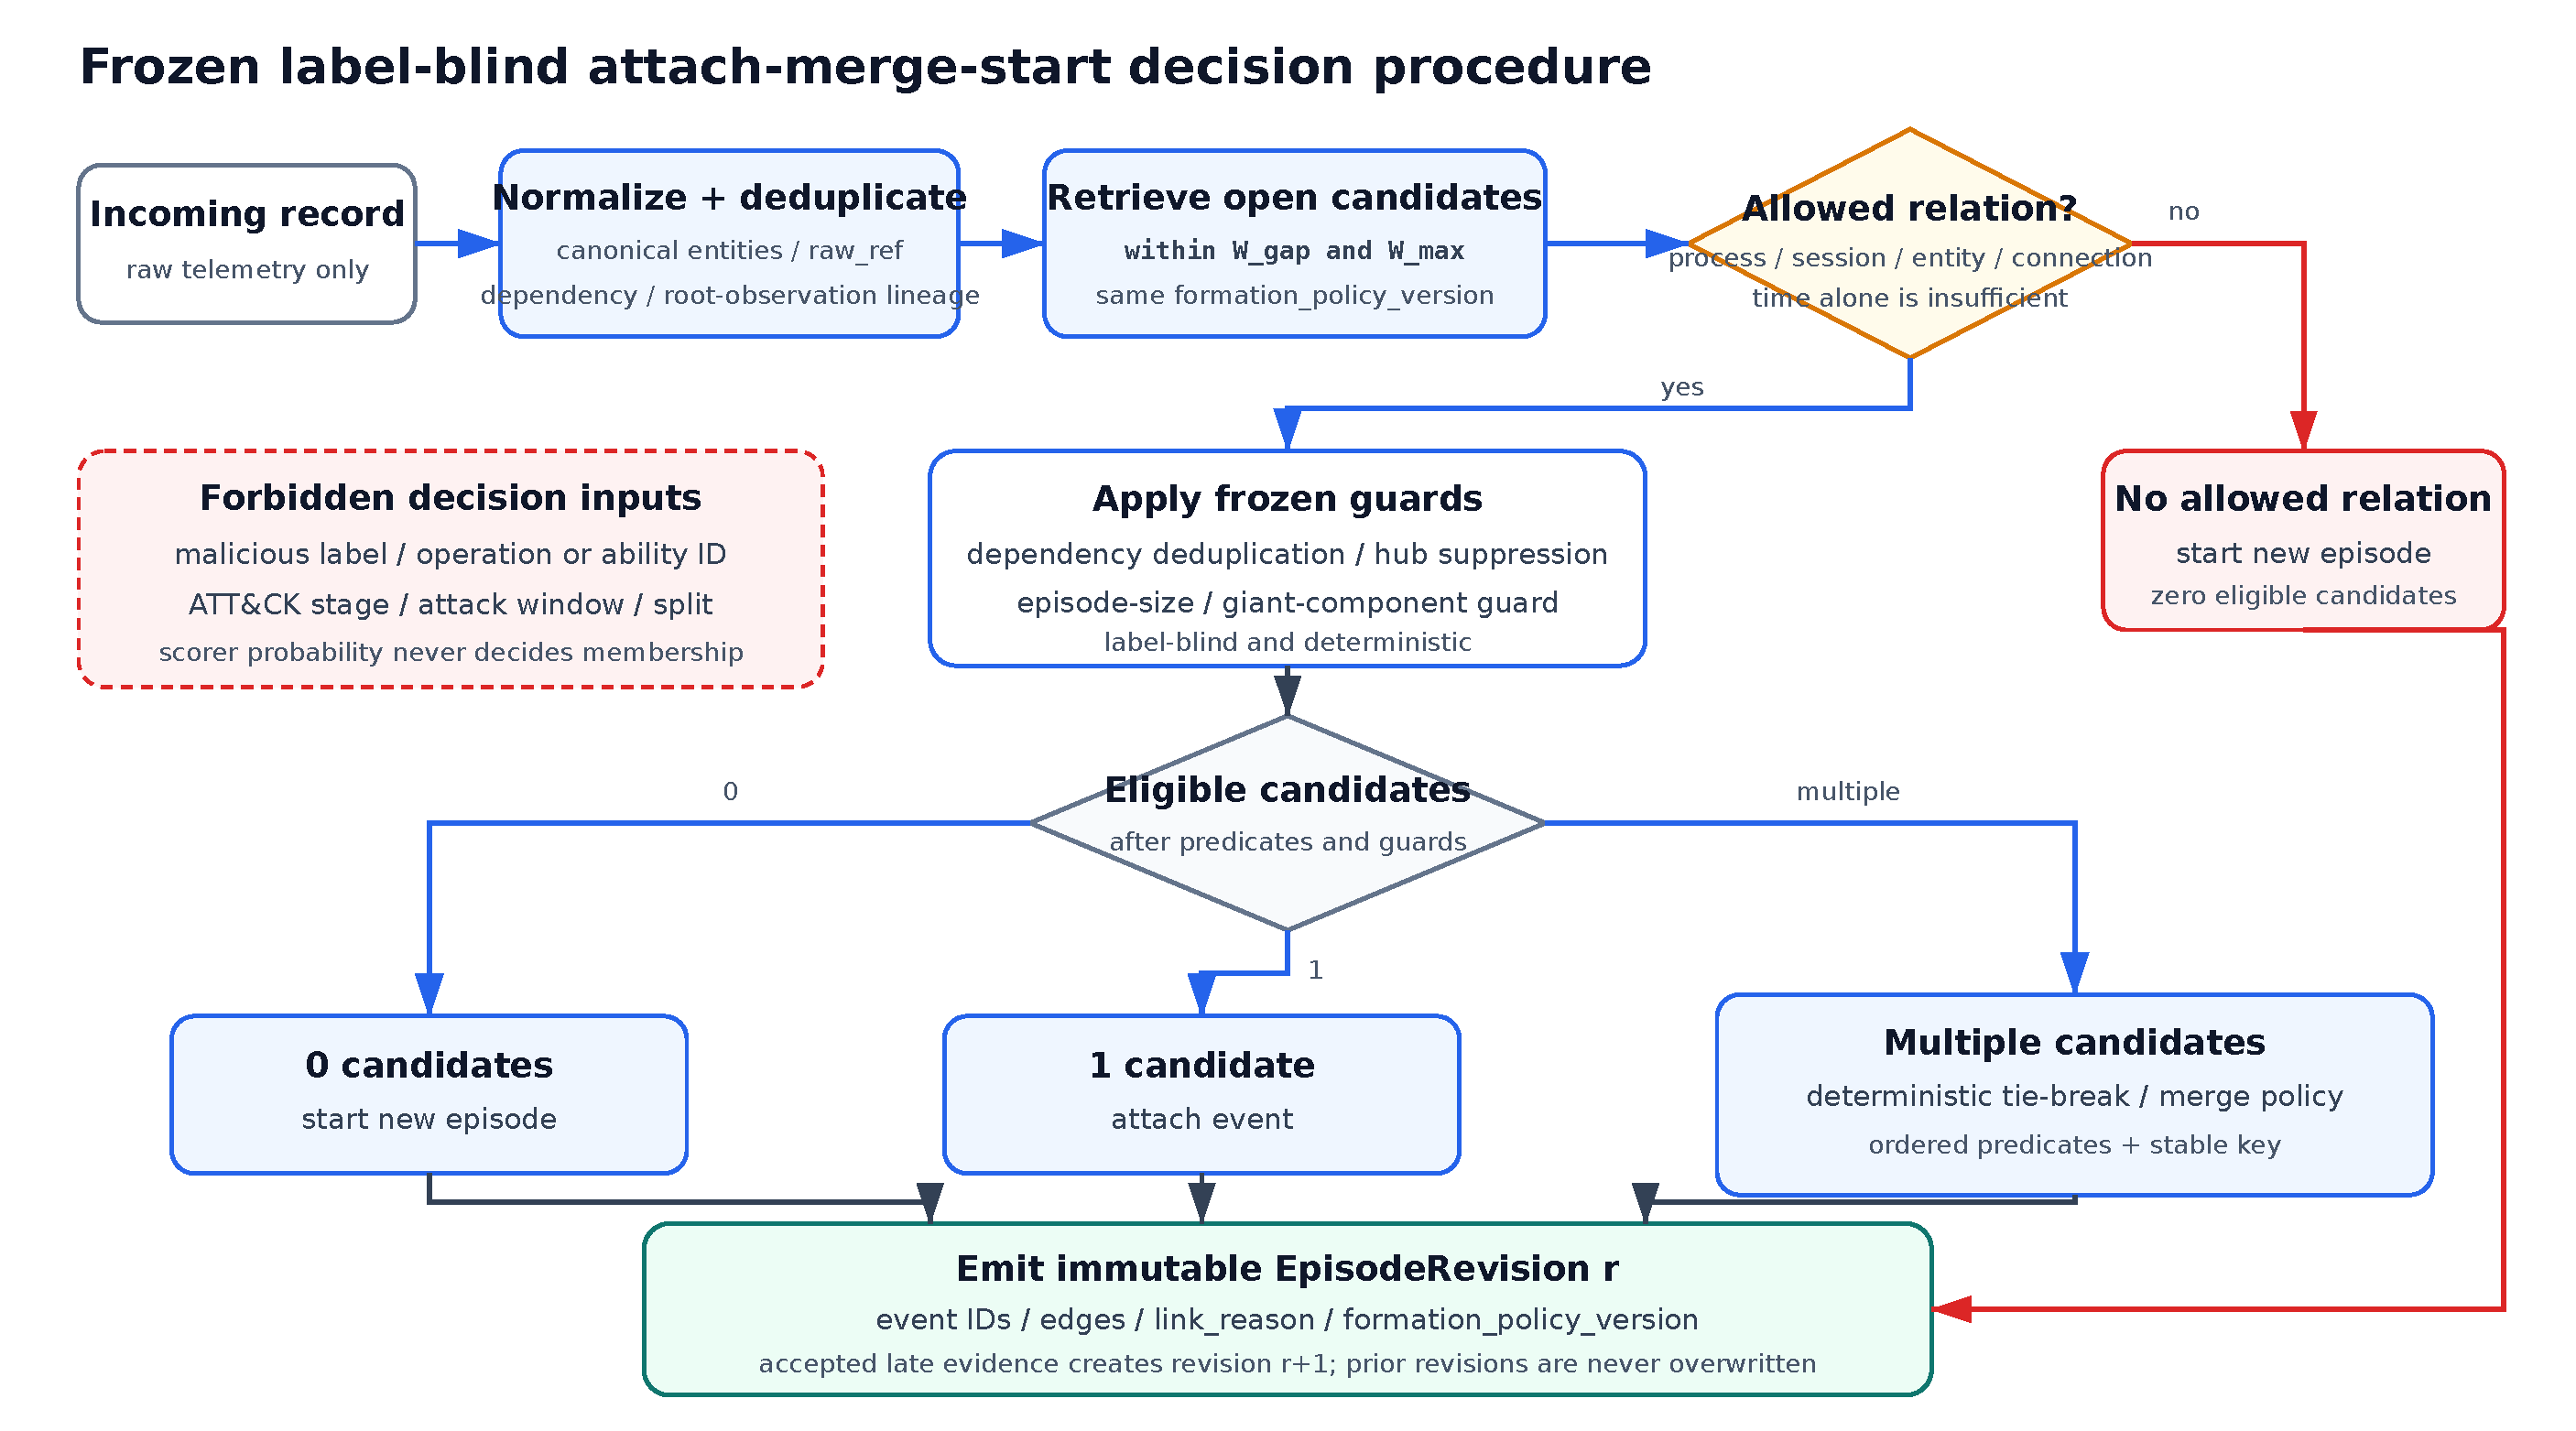
\includegraphics[width=\textwidth]{trustepisode_figures/pdf/fig08_episode_linking_decision.pdf}
  \caption{Frozen label-blind attach--merge--start procedure. Candidate retrieval, relation
  checks, guards, and total ordering execute before Episode Synthesis emits a revision; labels
  and scorer outputs cannot influence membership.}
  \label{fig:episode-linking-decision}
\end{figure*}

\subsection{Inclusive Eligibility and Allowed Relations}

Both temporal comparisons in Equation~\ref{eq:link-eligibility} are inclusive with
$W_{\mathrm{gap}}=300$ s and $W_{\max}=3600$ s:
$\Delta_t=W_{\mathrm{gap}}$ and $\operatorname{span}(E\cup\{e_i\})=W_{\max}$ remain eligible. Values larger than either bound
are ineligible. The relation predicate $R$ is true when at least one of the following frozen,
namespace-aware relations holds:
\begin{enumerate}[leftmargin=*,itemsep=1pt,topsep=2pt]
\item process parent-child or process-to-file causal continuity;
\item authenticated local/remote session continuity;
\item a network connection with a specific source/destination endpoint mapping;
\item the same non-generic host, user, process, file, service, or session entity.
\end{enumerate}
The hub predicate $H$ is true when all apparent support is attributable only to an entity with
at least 25 distinct relations in the preceding 600 s. Dependency-linked duplicates are
collapsed before $R$ and $H$ are evaluated.

\subsection{Total Order and Branch Semantics}

Candidate episodes are ordered by the tuple
\begin{equation}
(-\rho,-n_R,\Delta_t,t_{\mathrm{start}},\mathrm{episode\_id}),
\label{eq:candidate-order}
\end{equation}
where $\rho$ is the strongest relation precedence, $n_R$ is the number of distinct allowed
relation classes, $\Delta_t$ is the smallest event-time gap, $t_{\mathrm{start}}$ is episode
start time, and the final key is lexical. Relation precedence is process-causal, authenticated
session, endpoint-mapped connection, then specific-entity equality. This tuple is the only
tie-break order.

With zero eligible candidates, the builder starts an episode whose ID is the SHA-256 digest of
the formation-policy version, first event ID, and canonical namespace. With one candidate, it
attaches the event. With multiple candidates, it merges only when there are at most three
parents, every parent is connected through the new event by a process-causal, authenticated-
session, or endpoint relation, and the result has at most 500 events and 200 entities;
otherwise it attaches to the first ordered candidate. A merge ID is the digest of the literal \texttt{merge}, the sorted parent IDs, and
the formation-policy version. Parent IDs and their last revision numbers are retained as merge
lineage.

Within a revision, events are ordered by
\begin{equation}
(t^{event},t^{ingest},
\mathrm{source\_instance},\mathrm{event\_id}).
\end{equation}
The revision digest
covers the canonical episode ID, revision number, ordered membership, ordered link reasons,
lineage, and formation-policy version. These rules eliminate dependence on thread scheduling
or database return order.

\subsection{Watermark and Late Evidence}

The watermark is maximum observed ingest time minus $L_{\mathrm{wm}}=120$ s. An episode moves
\texttt{open}$\rightarrow$\texttt{finalized} when its event-time end precedes the watermark;
this freezes $t_f$ and deadline $t_f+W_{\mathrm{rev}}$. Accepted evidence before the deadline
emits a finalized successor without reopening or extending the horizon. At the deadline a
membership-identical closed successor is emitted; later evidence creates only a
LateEvidenceRecord in the late store and cannot alter history. Event time is never
overwritten to make late evidence appear timely.

\subsection{Deterministic Procedure and Replay Test}

\begin{enumerate}[leftmargin=*,itemsep=1pt,topsep=2pt]
\item Validate the NormalizedEvent schema and deduplicate by root dependency group.
\item Retrieve open episodes whose inclusive time bounds can admit the event.
\item Compute allowed relation classes and reject hub-only support.
\item Apply the 3-parent, 500-event, 200-entity, and strong-relation merge guards.
\item Sort candidates exactly by Equation~\ref{eq:candidate-order}.
\item Execute the zero/one/multiple branch and construct canonical lineage.
\item Order membership, compute the revision digest, and emit EpisodeRevision.
\item Compute $D,C,m,o^{det},z$; resolve $a^{det},\kappa,g,e$ from SourceCoverage; then compute $P,U$.
\item Join exact keys/versions and insert one AuditRecord or terminal AssemblyFailureRecord.
\item Advance the watermark; emit accepted successors or a beyond-horizon LateEvidenceRecord.
\end{enumerate}

The replay test runs the same normalized input twice under different worker counts and
database insertion orders. It compares episode/revision IDs, ordered memberships, link
reasons, lineage, features, scores, statuses, $U$, evidence references, and canonical digests.
Any mismatch is a correctness failure, not measurement noise.

\section{Feature, Sufficiency, and Parameter Registry}
\label{app:parameter-registry}

\subsection{Feature and Supporting-Evidence Contract}

For source family $s$, the empirical CDF artifact
$\widehat F^{\mathrm{train,benign}}_s$ is fit on training-benign detector values after source
parser validation. Ties use the right-continuous empirical CDF. The artifact records sample
count, fitting window, source contract, parser version, and content hash. Episode-level
$D_\epsilon$ is the arithmetic mean of the three greatest eligible transformed values. The
fixed top-three constant is not learned.

$q_{\epsilon,s}=1$ requires an upstream detection record with an immutable raw pointer, root
dependency group, detector-contract version, and a verified relation to an episode core entity
or edge. Coverage heartbeat, inventory, unscored raw presence, and another transport of the
same root observation are ineligible. The primary corroboration feature remains
$C=q_{\mathrm{EDR}}q_{\mathrm{NDR}}$ with fixed $K=2$.

Feature Extractor emits only health-independent \texttt{detected},
\texttt{examined\_none}, or \texttt{not\_examined}, together with $m$. Scope Resolver combines
these with the unique covering SourceCoverage interval to emit \texttt{available},
\texttt{no\_detection}, \texttt{collector\_unavailable}, \texttt{parser\_invalid}, or
\texttt{unknown}. Only the first two are support eligible; missing states force out-of-support
and are never interpreted as negative evidence.

\subsection{Complete Sufficiency Rules}

\begin{table*}[t]
\caption{Complete deterministic rules for $U$.}
\label{tab:u-registry}
\centering
\scriptsize
\begin{tabular}{p{0.14\textwidth}p{0.22\textwidth}p{0.56\textwidth}}
\toprule
\textbf{Axis} & \textbf{Value} & \textbf{Rule} \\
\midrule
coverage & unknown & first: any required health interval is missing or conflicting \\
 & unavailable & else any expected instance is down/not collected or any parser is invalid \\
 & degraded & else at least one expected instance is degraded \\
 & complete & else every expected instance is healthy and parser valid \\
\midrule
provenance & missing & first: any scored value, accepted link, membership event, or required root is unresolved \\
 & partial & else at least one optional unscored reference is absent \\
 & complete & else every required pointer and dependency root resolves \\
\midrule
lateness & late-accepted & first: this revision was created by accepted late evidence \\
 & revisable & else episode is open or finalized inside the 900 s horizon \\
 & stable & else episode is closed \\
\midrule
contradiction & present & first: CR1 endpoint binding, CR2 normalized flow direction, or CR3 process lineage conflict is true \\
 & unevaluable & else any applicable rule lacks required online input \\
 & none & else every applicable frozen online rule is false \\
\midrule
calibration & \texttt{supported\_global} & $\kappa=\texttt{supported\_global}$ \\
 & \texttt{supported\_group} & $\kappa=\texttt{supported\_group}$ \\
 & \texttt{out\_of\_support} & $\kappa=\texttt{out\_of\_support}$ \\
\bottomrule
\end{tabular}
\end{table*}

CR1 tests overlapping authenticated endpoint bindings for different hosts; CR2 tests matched
EDR socket/NDR flow initiator disagreement after direction normalization; CR3 tests conflicting
parent/root lineage for one $(host,boot,pid,start)$ key. A rule is applicable only when its
relation exists; missing required fields then yield \texttt{unevaluable}, while no applicable
relation yields \texttt{none}. These rules cannot read a Caldera operation, ability, attack
window, scenario, split, or offline label. The five axes are never converted to one number.

\begin{figure*}[t]
  \centering
  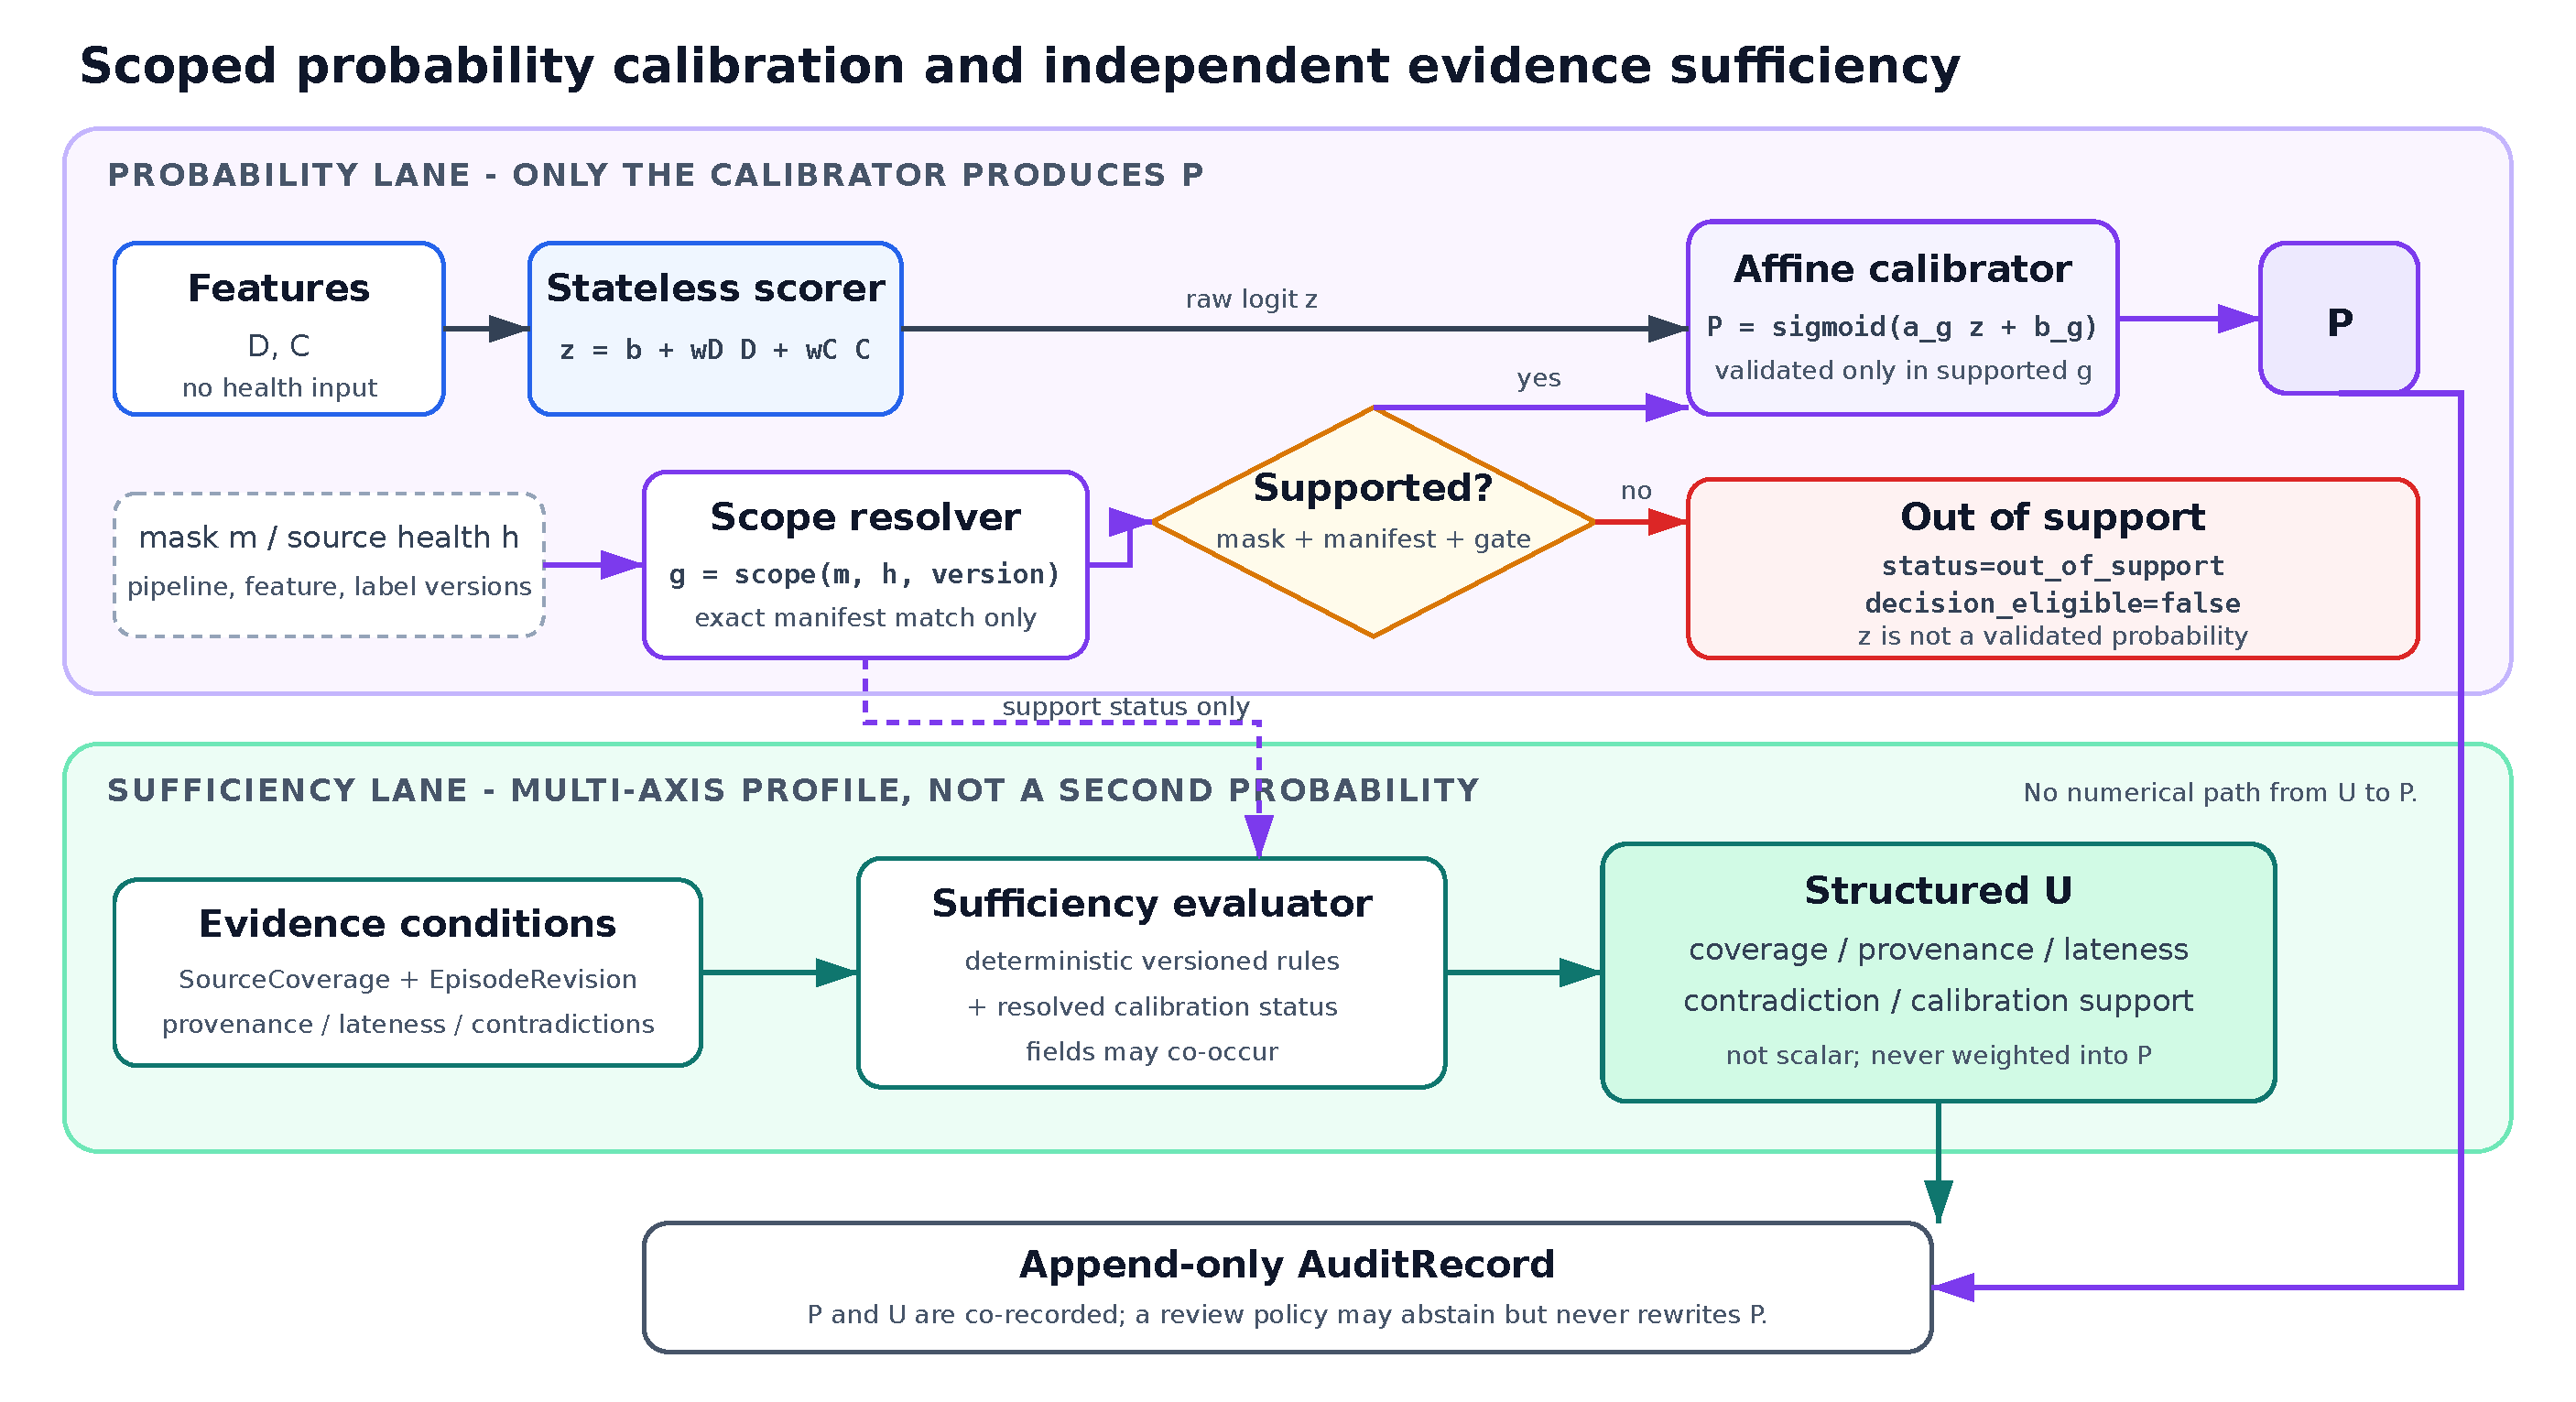
\includegraphics[width=\textwidth]{trustepisode_figures/pdf/fig03_calibration_and_sufficiency.pdf}
  \caption{Probability calibration and evidence sufficiency are independent lanes. Detector
  state participates in support resolution, while $U$ has no numerical path into $P$; the
  AuditRecord Assembler emits one terminal AssemblyOutcome to a sink-only store.}
  \label{fig:calibration-sufficiency-companion}
\end{figure*}

\subsection{Parameter Taxonomy}

\begin{table*}[t]
\caption{Parameter and state taxonomy.}
\label{tab:parameter-taxonomy}
\centering
\scriptsize
\begin{tabular}{p{0.13\textwidth}p{0.17\textwidth}p{0.07\textwidth}p{0.13\textwidth}p{0.16\textwidth}p{0.16\textwidth}}
\toprule
\textbf{Category} & \textbf{Content} & \textbf{Learned?} & \textbf{Owner} & \textbf{Selection/fit data} & \textbf{Freeze point} \\
\midrule
Scorer coefficients & $(b,w_D,w_C)$ & yes & Stateless Scorer & training fit; development selects contract & before calibration \\
Global calibrator & $(a,b_{\mathrm{cal}})$ & yes & Calibrator & natural-prevalence calibration split & before locked test \\
Conditional calibrator & $(a_g,b_g)$ & yes & Calibrator & calibration run folds after gate & before locked test \\
Formation policy & time, revision, hub, component, merge settings & no & Episode Synthesis & training/development & before final train-only fit \\
Fixed aggregation & top three; primary $K=2$ & no & Feature contract & method specification & before training \\
Evidence state & $m,h,q,a^{det}$ & no & Table~\ref{tab:ownership} producers & runtime observation & per revision \\
Output/status & $\kappa,U$ & no & Scope/Sufficiency Evaluators & deterministic runtime rules & per AuditRecord \\
Version metadata & schema, policy, model, calibrator, manifest hashes & no & Artifact Registry & producing artifact's split & artifact publication \\
Evaluation settings & split seed, perturbations, bootstrap repetitions & no & Evaluation Harness & pilot/development preregistration & before locked test \\
\bottomrule
\end{tabular}
\end{table*}

The unconditional primary method therefore has five fitted scalar coefficients:
$\{b,w_D,w_C,a,b_{\mathrm{cal}}\}$. Empirical CDFs are frozen fitted preprocessing artifacts,
not fixed constants. Conditional group coefficients exist only for groups that pass the
registered gate.

\subsection{Single Threshold Registry}

Every threshold is defined only in Table~\ref{tab:threshold-registry}; other sections refer to
its symbol and owner.

Primary values are $W_{\mathrm{gap}}=300$ s, $W_{\max}=3600$ s,
$W_{\mathrm{rev}}=900$ s, $L_{\mathrm{wm}}=120$ s, $f_{\mathrm{hub}}=25$ distinct
relations per 600 s, and $n_{\mathrm{component}}=(500\text{ events},200\text{ entities})$.
Label/matching values are $\theta_{\mathrm{mal}}=.50$,
$\theta_{\mathrm{contam}}=.25$, and $\theta_{\mathrm{match}}=.50$ with minimum time IoU .10
and entity Jaccard .50. The group gate fixes
$(n_{\mathrm{pos}}^{\min},n_{\mathrm{neg}}^{\min},n_{\mathrm{run}}^{\min})=(50,50,10)$,
five run folds, and minimum mean Brier/NLL improvements $(.01,.01)$ with positive paired 95\%
lower bounds. Values are mirrored in \path{thresholds.v1.json}; a code/paper mismatch fails
artifact validation.

\begin{table*}[t]
\caption{Threshold ownership, selection, freeze, and validation registry.}
\label{tab:threshold-registry}
\centering
\scriptsize
\begin{tabular}{p{0.12\textwidth}p{0.25\textwidth}p{0.17\textwidth}p{0.16\textwidth}p{0.20\textwidth}}
\toprule
\textbf{Symbol} & \textbf{Meaning} & \textbf{Owner} & \textbf{Selection data} & \textbf{Freeze and validation} \\
\midrule
$W_{\mathrm{gap}}$ & maximum event-time inactivity gap & formation policy & development & before final train fit; EB1/EB2 sensitivity \\
$W_{\max}$ & maximum event-time episode span & formation policy & development & before final train fit; M7 sensitivity \\
$W_{\mathrm{rev}}$ & post-watermark revision horizon & revision policy & development/pilot & before calibration; delay replay \\
$L_{\mathrm{wm}}$ & allowed ingest lateness for watermark & revision policy & development/pilot & before calibration; delay replay \\
$f_{\mathrm{hub}}$ & generic/high-frequency entity cutoff & formation policy & training/development & before final train fit; EB3-H ablation \\
$n_{\mathrm{component}}$ & giant-component event/entity limit & formation policy & development & before final train fit; stress replay \\
$\theta_{\mathrm{mal}}$ & minimum malicious overlap for positive label & label policy & pilot/adjudication & before partitioned labels are released \\
$\theta_{\mathrm{contam}}$ & unrelated-benign overlap for mixed label & label policy & pilot/adjudication & before partitioned labels are released \\
$n_{\mathrm{pos}}^{\min}$ & minimum group-calibration positives & calibration gate & pre-registered before calibration & before group fitting; internal run folds \\
$n_{\mathrm{neg}}^{\min}$ & minimum group-calibration negatives & calibration gate & pre-registered before calibration & before group fitting; internal run folds \\
$n_{\mathrm{run}}^{\min}$ & minimum independent calibration runs & calibration gate & pre-registered before calibration & before group fitting; internal run folds \\
$\Delta_{\mathrm{miscal}}^{\min}$ & minimum validated global-calibration deficiency & calibration gate & pre-registered before calibration & internal run folds only \\
$\theta_{\mathrm{match}}$ & minimum action/entity overlap for episode matching & evaluation policy & development & before locked test; matching sensitivity \\
\bottomrule
\end{tabular}
\end{table*}

\section{Calibration Manifest, Eligibility, and Invalidation}
\label{app:calibration-manifest}

\subsection{Manifest Contract}

\begin{table*}[t]
\caption{Required calibrator-manifest fields.}
\label{tab:calibrator-manifest}
\centering
\scriptsize
\begin{tabular}{p{0.26\textwidth}p{0.63\textwidth}}
\toprule
\textbf{Field group} & \textbf{Required values} \\
\midrule
Candidate contract & formation-policy version; candidate-selection version; label-policy version \\
Feature contract & feature version; EDR/NDR detector-contract versions; empirical-CDF hashes; detector-state and missing-value contract \\
Model contract & raw-model version and digest; coefficient digest; training split manifest \\
Calibration contract & calibrator version; global coefficients; registered group-key fields/digests; eligible final-refit coefficients; calibration split manifest \\
Runtime support & exact source mask \texttt{11}; allowed health/detector states; schema/parser versions; deployment/pipeline version \\
Evidence and audit & calibration counts, prevalence as metadata, gate evidence, reliability-bin specification, manifest digest \\
\bottomrule
\end{tabular}
\end{table*}

Support requires exact equality for every contract field that affects candidate construction,
features, raw scores, or calibration meaning. The resolver never chooses a nearest source mask
or silently maps a novel pipeline version to an old artifact.

\subsection{Global and Conditional Group Resolver}

The global mapping uniquely minimizes natural-prevalence NLL plus
$10^{-6}(a^2+b_{\mathrm{cal}}^2)$ subject to $a\ge10^{-6}$. Primary support requires exact
mask \texttt{11}, no down/unknown health, valid parsers, and detector states
\texttt{available} or \texttt{no\_detection}. Each group key is pre-registered as the RFC~8785/
SHA-256 digest of deployment profile and EDR/NDR detector versions; scenario, run, identity,
and label fields are forbidden. A group is considered only with
at least 50 positives, 50 negatives, and 10 independent runs. Runs use deterministic five-fold
assignment with seed 20260710; each fold evaluates a mapping fitted on the other four. A group
is enabled only when mean held-out improvements in both Brier and NLL are at least .01, every
fold is nonnegative, and both paired run-bootstrap lower 95\% bounds exceed zero. Undefined or
tied gates fall back to global. Passing group coefficients are then refit on all calibration
records for the exact key and sealed in a duplicate-key-rejecting manifest; locked test never
selects or refits a group.

Resolution follows one exclusive branch:
\begin{enumerate}[leftmargin=*,itemsep=1pt,topsep=2pt]
\item Exact support plus one enabled exact group key:
      use $(a_g,b_g)$ and serialize \path{supported_group}.
\item Exact support without an enabled exact key:
      use $(a,b_{\mathrm{cal}})$ and serialize \path{supported_global}.
\item Any required manifest or supported-regime mismatch:
      serialize \path{out_of_support}, set $P=\texttt{null}$, and set
      \path{decision_eligible=false}.
\end{enumerate}
Group-gate failure is therefore distinct from out-of-support status.

\begin{figure*}[t]
  \centering
  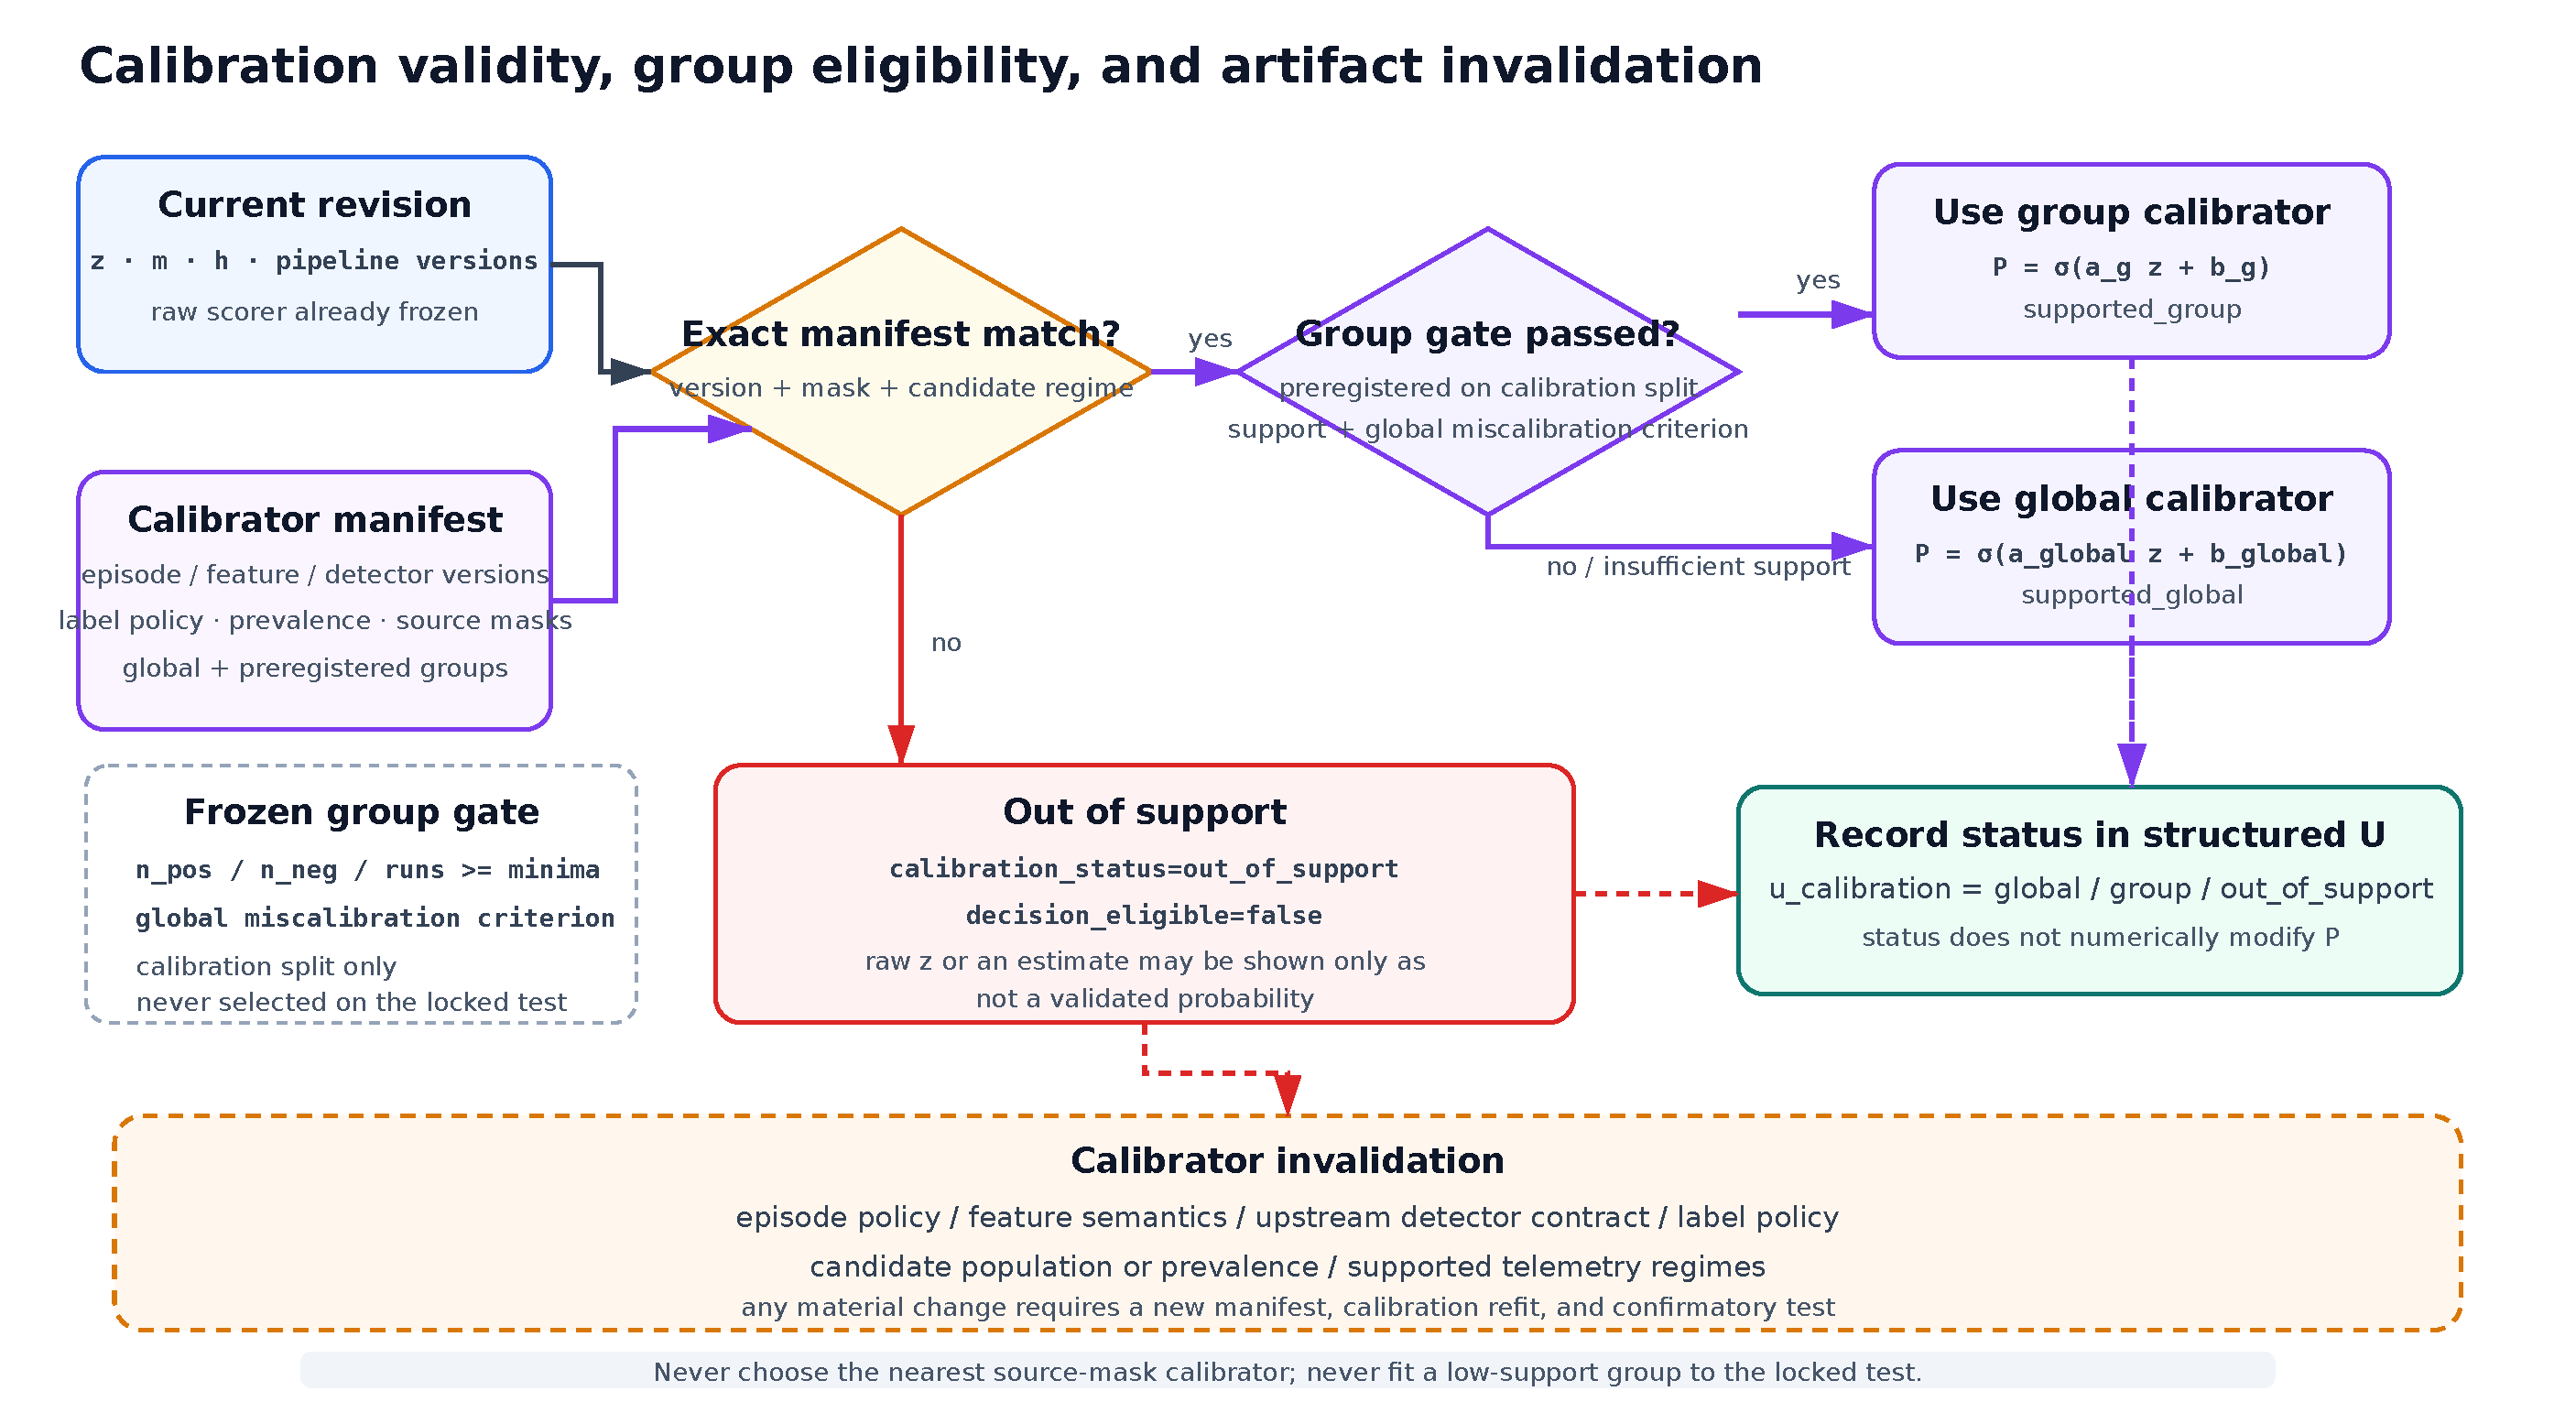
\includegraphics[width=\textwidth]{trustepisode_figures/pdf/fig09_calibration_validity_state_machine.pdf}
  \caption{Exclusive calibration resolution and invalidation. Exact source, health, detector,
  and version support is required; the five-fold group gate can only select between a
  registered group and global fallback, never manufacture support.}
  \label{fig:calibration-validity-companion}
\end{figure*}

\subsection{Invalidation Matrix}

\begin{table*}[t]
\caption{Calibrator invalidation and revalidation rules.}
\label{tab:calibrator-invalidation}
\centering
\small
\begin{tabular}{p{0.29\textwidth}p{0.30\textwidth}p{0.31\textwidth}}
\toprule
\textbf{Change} & \textbf{Immediate status} & \textbf{Required action} \\
\midrule
Episode policy or candidate-selection policy & invalid & rebuild candidates; refit scorer and calibrator \\
Feature semantics, normalizer, or missing rule & invalid & refit scorer and calibrator \\
Upstream detector contract or parser semantics & out of support & revalidate features; refit if distribution/meaning changes \\
Raw-model coefficients or training population & invalid & refit calibrator \\
Label policy & invalid for supervised claim & regenerate labels; repeat fit and evaluation \\
Supported source mask or health regime & out of support & collect calibration support and register a new manifest \\
Schema-only additive field excluded from features & pending compatibility check & prove canonical equivalence before manifest amendment \\
Candidate prevalence drift & revalidation signal only & audit reliability; do not automatically change episode-level output \\
\bottomrule
\end{tabular}
\end{table*}

Prevalence is recorded because it affects interpretation and may motivate revalidation, but an
unknown current deployment prevalence is never an online per-revision gate. Out-of-support
records expose $z$ only with raw-logit wording and serialize $P$ as canonical null under
Appendix~\ref{app:canonical-serialization}.

\section{Laboratory, Ground Truth, and Label Policy}
\label{app:lab-label-policy}

\subsection{Run and Environment Manifest}

Every formal run stores: run and pair IDs; scenario and benign-workload manifest versions;
Caldera v5.3.0 annotated tag object
\texttt{dd22d543a519afe63ca35c454bf1add5d75c45dc}, peeled commit
\texttt{b24f6e7a99cab19cbf417009bda9b9c6c81abc31}; target image SHA-256 hashes;
VM and network topology versions;
EDR/NDR collector images and configuration hashes; Health Monitor version; parser/schema
versions; clock source and maximum observed skew; random seed; start/end times; harmless
marker IDs; cleanup status; and any collection incident. Formal evaluation has no public-data
tier: provenance datasets remain related-work context because they do not implement the frozen
EDR/NDR collection contract. Formal results group by this run ID, not by Caldera ability or
individual episode. The complete machine contract is
\path{artifacts/contracts/lab_manifest.v1.json}; a missing required field fails closed.

\begin{figure*}[t]
  \centering
  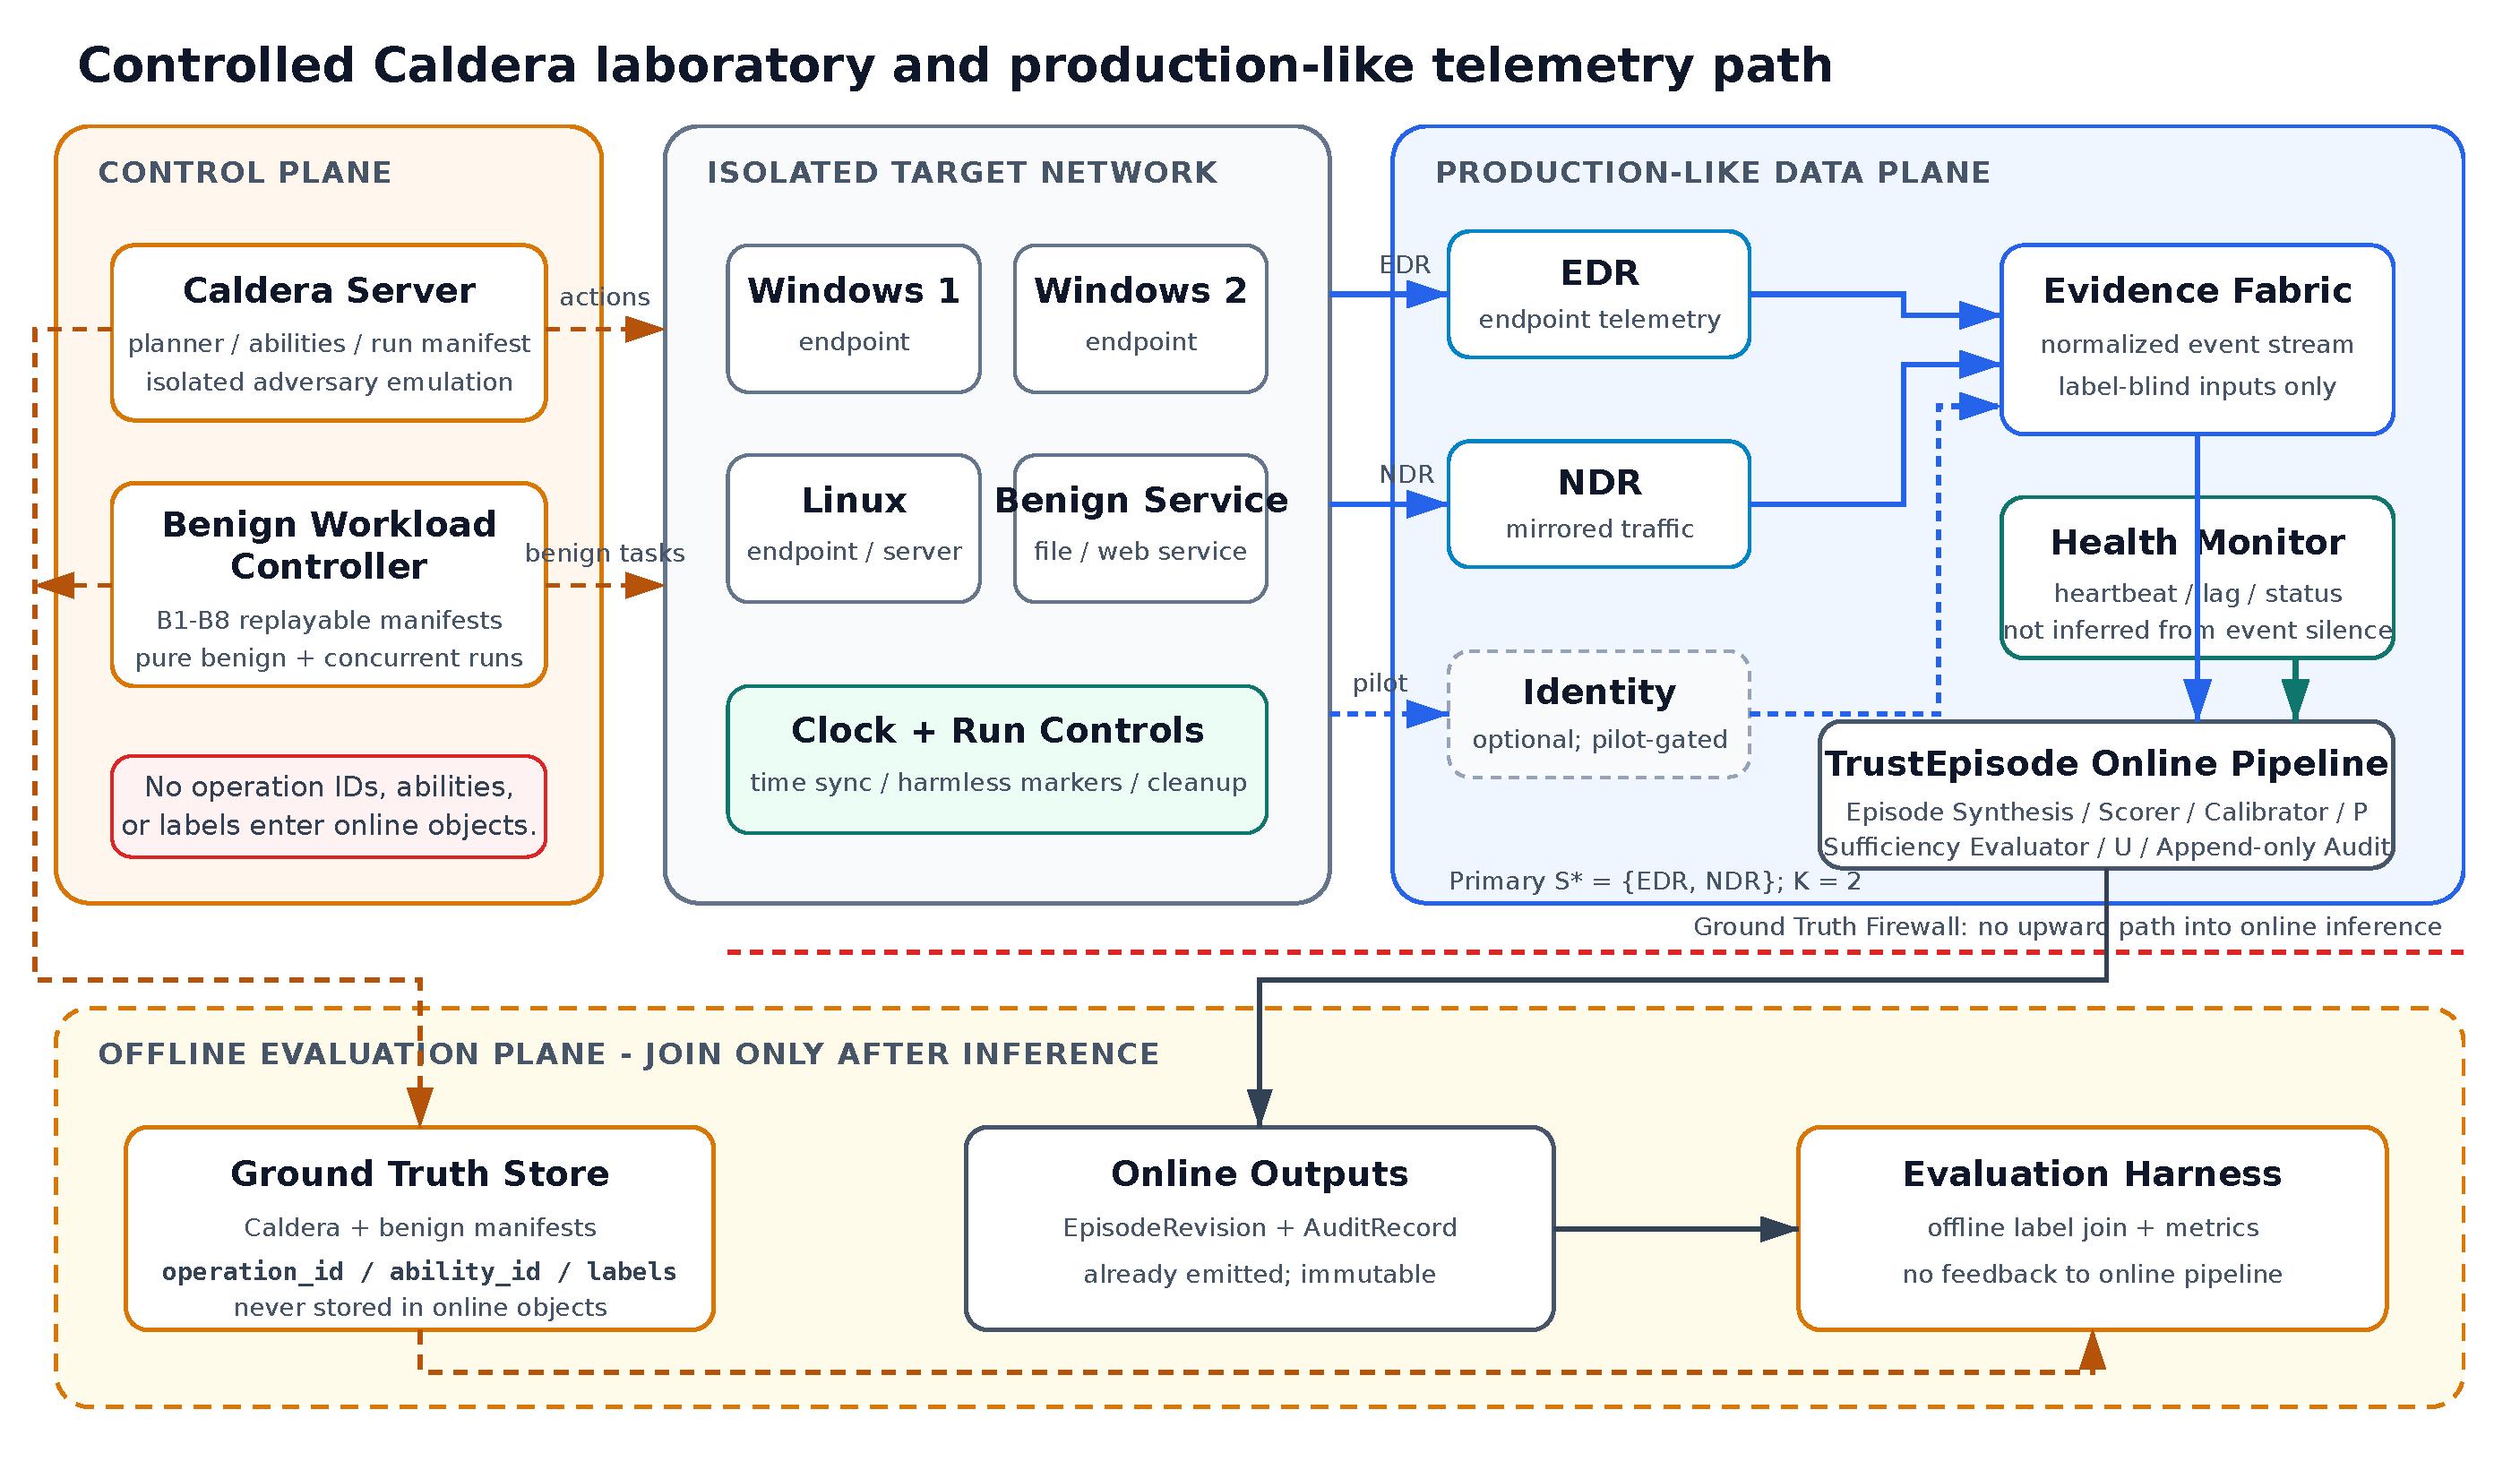
\includegraphics[width=\textwidth]{trustepisode_figures/pdf/fig04_lab_topology.pdf}
  \caption{Controlled laboratory topology. EDR and NDR are the only online telemetry sources;
  Identity is excluded from the candidate path and M5-ID can join only in offline evaluation.}
  \label{fig:lab-topology-companion}
\end{figure*}

\subsection{Scenario Cards and Failure Rules}

\begin{table*}[!t]
\caption{Malicious scenario-card registry. Actions use only isolated targets and harmless
per-run markers.}
\label{tab:scenario-cards}
\centering
\scriptsize
\begin{tabular}{p{0.05\textwidth}p{0.34\textwidth}p{0.28\textwidth}p{0.23\textwidth}}
\toprule
\textbf{ID} & \textbf{Precondition and ordered actions} & \textbf{Marker and expected observations} & \textbf{Cleanup and card-specific failure} \\
\midrule
M1 & two Windows targets and test share; discovery $\rightarrow$ share access $\rightarrow$ test-account remote execution & unique process/file marker; EDR lineage plus NDR remote connection & remove marker/session/service; abort if either primary collector fails \\
M2 & Windows target; script execution $\rightarrow$ staged marker transfer $\rightarrow$ temporary scheduled-task persistence & script/process/file marker; EDR lineage and NDR transfer & delete task and marker; record inability to remove persistence as cleanup failure \\
M3 & Linux targets; discovery $\rightarrow$ test-account SSH $\rightarrow$ marker file action & shell/file marker; Linux EDR lineage and NDR SSH flow & terminate shell, revoke key, remove marker; abort on namespace mismatch \\
M4 & instrumented service; low-rate periodic connections $\rightarrow$ local marker action & seeded connection cadence plus EDR local action & stop client and remove marker; fail card if cadence manifest is not replayed \\
M5 & test-account endpoint action $\rightarrow$ endpoint marker & EDR/NDR primary evidence independent of Identity & revoke credential and marker; fail if either primary collector is unhealthy \\
M6 & dual-use administration tool also present in benign cards; contextual misuse $\rightarrow$ remote marker action & identical tool name in both classes; sequence/context plus EDR/NDR distinguish use & remove marker/session; preserve unsuccessful execution as declared failure \\
M7 & extended schedule; discovery $\rightarrow$ frozen pauses $\rightarrow$ remote action $\rightarrow$ marker & weak observations across $W_{\mathrm{gap}}$/$W_{\max}$ boundaries & terminate sessions/markers; report any schedule-bound violation \\
\bottomrule
\end{tabular}
\vspace{8pt}
\caption{Benign and hard-negative workload-card registry.}
\label{tab:benign-cards}
\centering
\scriptsize
\begin{tabular}{p{0.05\textwidth}p{0.34\textwidth}p{0.28\textwidth}p{0.23\textwidth}}
\toprule
\textbf{ID} & \textbf{Precondition and ordered actions} & \textbf{Expected observations} & \textbf{Cleanup and card-specific failure} \\
\midrule
B1 & approved PowerShell/bash inventory over registered targets & process, query, and normal connection evidence & remove output; fail if command leaves target state changed \\
B2 & signed test patch deployment and verification & installer lineage, package writes, repository flow & uninstall/revert snapshot; record reboot or rollback failure \\
B3 & seeded file-share synchronization of benign fixtures & burst file operations and SMB/NFS flows & remove synchronized fixtures; verify checksums \\
B4 & authorized vulnerability scan against isolated service & high fan-out NDR flows and expected service logs & stop scanner; fail if target leaves healthy state \\
B5 & helpdesk test-account remote administration & same remote/admin tools used in M1/M6 without malicious marker & terminate session and revoke temporary grant \\
B6 & scheduled log collection and forwarding & repeated reads, compression, and collector-bound network flow & remove bundle; verify no collector backlog \\
B7 & configuration-management convergence to a known benign state & remote orchestration, file/service updates, expected restart & restore baseline; fail on manifest drift \\
B8 & unscheduled but declared maintenance with a frozen work order & realistic administrative sequence with healthy EDR/NDR & verify service state; retain timing as hard-negative context \\
\bottomrule
\end{tabular}
\end{table*}

Every card records its version, target images, benign mode, repetition ID, and seed. Each
malicious family has exactly 10 successful attack-only repetitions and 10 successful
concurrent-benign repetitions; B1--B8 each have exactly 10 successful pure-benign repetitions.
The machine-readable ordered actions, markers, observations, cleanup, and failure rules are in
\path{artifacts/contracts/scenario_cards.v1.json}. A collection failure excludes the run from
primary metrics but remains in RT1 and the failure log. A failed scenario action
with healthy primary collectors remains in the registered sensitivity view but not the
successful-run cohort. Cleanup failure blocks the next run on that image. No failed or aborted
run is silently reused under the same ID.

\subsection{Identity Pilot Gate}

Identity remains conditional under the separately registered M5-ID card. Before any
Identity-side analysis, pilot runs must demonstrate complete
timestamp alignment, stable benign and malicious capture, independent source health, raw
provenance pointers, and sufficient run-level support. Identity is always excluded from
NormalizedEvent, Episode Synthesis, candidate IDs and membership, $D,C,z$, every calibrator
manifest, and primary RQs. Gate failure suppresses all Identity-side reporting. Gate passage
permits only a separately labeled offline exploratory annotation after primary inference; it
cannot change the EDR/NDR candidate universe or $K=2$ contract.

\subsection{Ground Truth Store and Offline Join}

The Ground Truth Store uses a separate database role. Join keys are run ID, harmless marker
ID, target entity namespace, and versioned time interval. The Evaluation Harness first verifies
that online inference and AuditRecord insertion have completed, then performs the join under
the frozen label-policy digest. A two-reviewer adjudication resolves disagreements; unresolved
cases become ambiguous rather than being forced into the binary cohort.

Offline matching first requires temporal IoU at least $.10$, entity Jaccard at least $.50$,
and one exact harmless marker or registered action. Within one run, maximum-weight bipartite
assignment uses
$w=.5A_{cov}+.3J_{entity}+.2\operatorname{IoU}_{time}\ge\theta_{match}=.50$;
ties use entity overlap, absolute time difference, then lexical IDs. A revision is positive
when malicious-action coverage is at least $\theta_{mal}=.50$ and unrelated benign
contamination is below $\theta_{contam}=.25$; mixed when both thresholds are met; negative when
malicious coverage is zero and activity has registered benign/background attribution; all
residual, missing, or conflicting cases are ambiguous. Labels are revision specific and join
only after AuditRecord insertion. Sensitivity varies $\theta_{mal}\in\{.25,.50,.75\}$,
$\theta_{contam}\in\{.10,.25,.50\}$, and $\theta_{match}\in\{.40,.50,.60\}$ without altering
the primary registry after seeing performance.

\subsection{Leakage Tests}

Continuous schema tests inject each forbidden field into every online object and require a
hard rejection. Partition tests verify that every descendant of one run has exactly one split.
Feature-lineage tests prove that all scorer inputs trace to allowed online fields. SQL-role
tests deny online reads from Ground Truth Store tables. A canary scenario token is placed only
in the offline store and must be absent from every normalized event, revision, feature, model
input, and AuditRecord. Any failure invalidates the affected run and blocks locked evaluation.

\clearpage
\section{Experimental Contract and Reproducibility}
\label{app:experimental-contract}

\subsection{Split and Freeze Manifest}

The registered views prevent revision multiplicity from changing a claim. $\mathcal C_{form}$
contains one terminal revision per surviving lineage at
$T_{form}=t_{run\_end}+L_{wm}+W_{rev}=t_{run\_end}+1020$ s, after removing merged parents.
$\mathcal C_{dec}$ contains the first finalized, decision-eligible revision per terminal
episode and is the only primary RQ2 population. $\mathcal C_{stream}$ contains every
AuditRecord keyed by $(episode\_id,revision)$ and is used only for RQ3/RQ4 transitions and
cost.

The independent split unit is a base campaign, stratified by scenario family and benign mode.
Within each stratum, campaigns sort by ascending SHA-256 of
\texttt{20260710:base\_campaign\_id}. In each consecutive 20-run cycle, ranks 0--9 are
training, 10--13 development, 14--16 calibration, and 17--19 locked test, targeting
50/20/15/15 percent. Replay and outage descendants inherit partition and bootstrap cluster;
any mismatch invalidates the complete cluster. The registry requires run, base, parent, and
pair IDs; scenario; benign mode; seed; partition; cluster; role; and manifest digest. The
freeze manifest additionally binds code, container/image, formation, feature, normalizer,
scorer, calibrator, label, baseline, intervention, metric, bin, and analysis-script digests.
The machine policy is \path{artifacts/contracts/split_policy.v1.json}; no post-label manual
balancing is permitted.

\begin{figure*}[t]
  \centering
  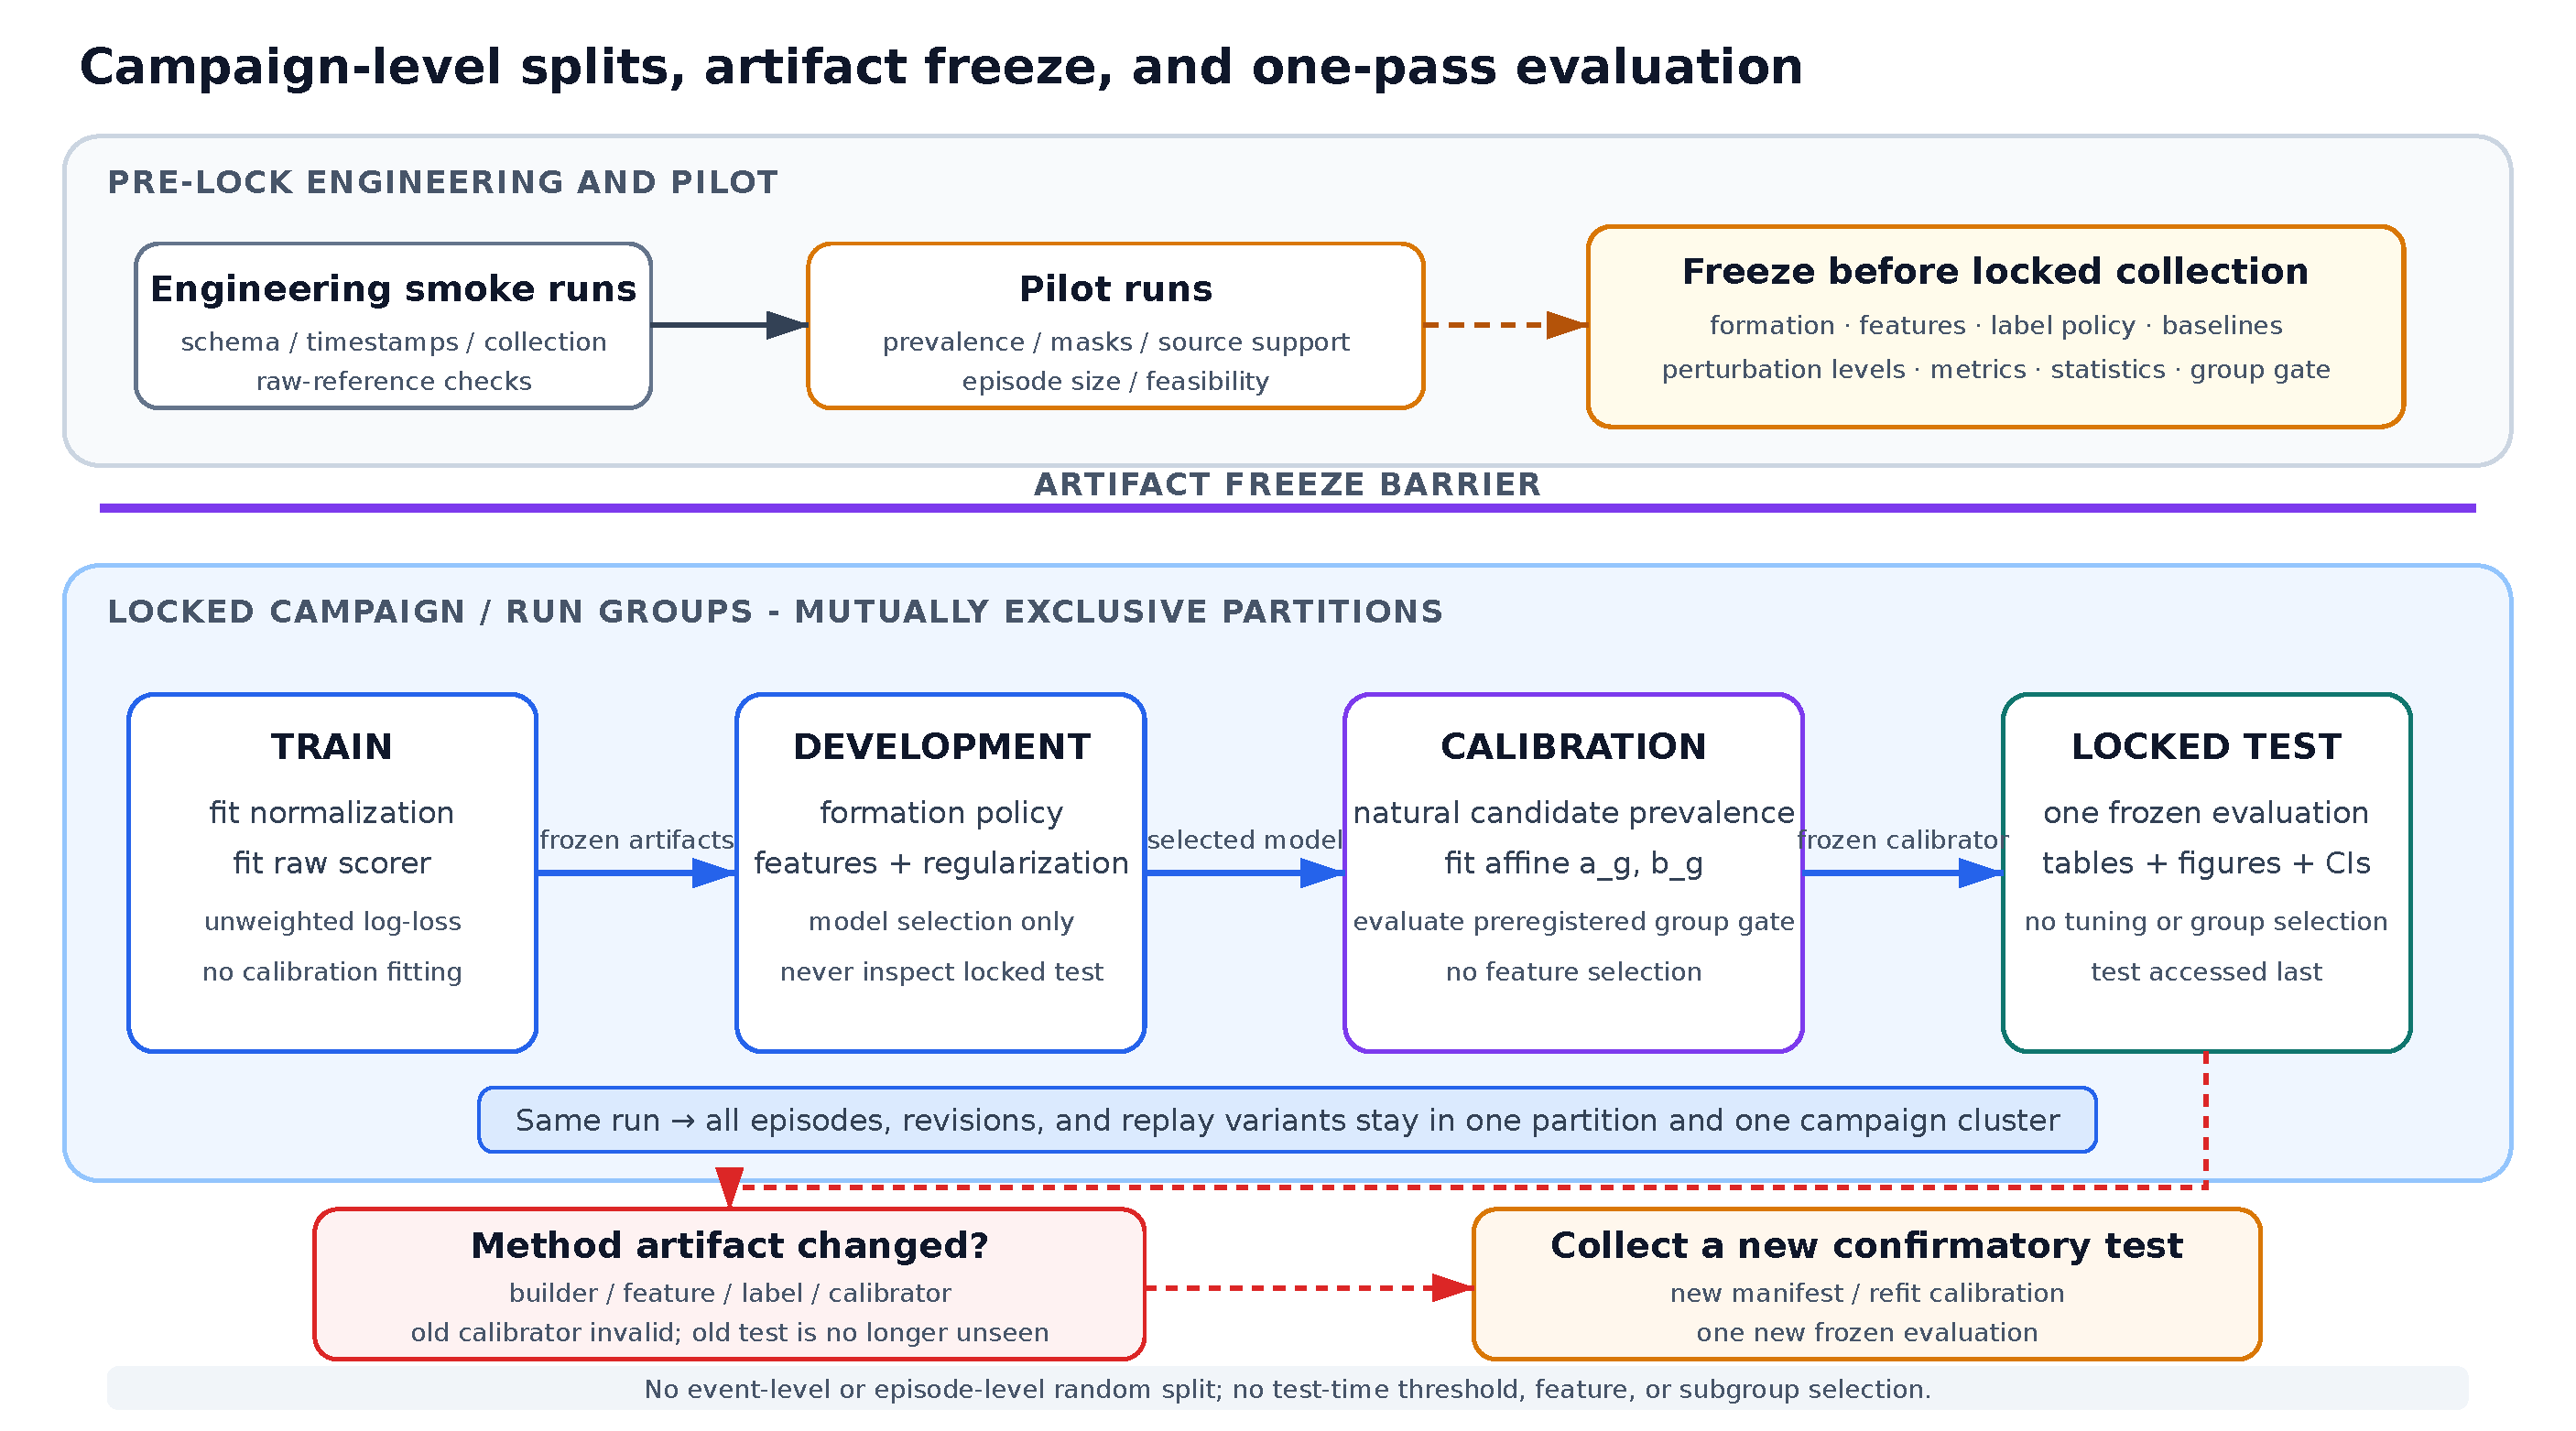
\includegraphics[width=\textwidth]{trustepisode_figures/pdf/fig06_split_and_freeze_workflow.pdf}
  \caption{Campaign-level split and freeze workflow. Deterministic 50/20/15/15 assignment is
  performed before label release, and all descendants inherit the base campaign partition and
  bootstrap cluster.}
  \label{fig:split-freeze-companion}
\end{figure*}

\subsection{Baseline Implementation Registry}

EB1 uses non-overlapping event-time windows of width $W_{\mathrm{gap}}$ with no entity or
causal merge. EB2 adds the requirement that consecutive records share one specific,
non-generic entity. EB3 is Algorithm~1; EB3-H changes only hub suppression. SB1 is the maximum
source-normalized vendor severity among eligible episode records. SB2 fits the same constrained
logit procedure as Equation~\ref{eq:raw-logit} with $w_C=0$. SB3 is the proposed raw logit.
SB4 reports the uncalibrated sigmoid score $\sigma(z)$ and is not called a probability. SB5
applies the global affine calibrator. SB6 is the
conditional group mapping. SB7 maps an unavailable source's absent detector value to zero and
ignores manifest support. OB1 is the physical-outage-only available-source denominator and
returns no corroboration when fewer than two source families are healthy. No entry has an
alternative max/mean, weight set, model capacity, or post-test implementation.

\subsection{Frozen Perturbation Grid and Outage Procedure}

\begin{table*}[t]
\caption{Pre-registered replay perturbations. Each variant includes an unchanged control and
uses a deterministic child seed derived from the base-run ID.}
\label{tab:perturbation-grid}
\centering
\small
\begin{tabular}{p{0.08\textwidth}p{0.21\textwidth}p{0.27\textwidth}p{0.33\textwidth}}
\toprule
\textbf{ID} & \textbf{Intervention} & \textbf{Frozen levels} & \textbf{Invariant} \\
\midrule
RP0 & unchanged replay & no mutation & exact canonical-hash equality required \\
RP1 & source-event mask & EDR only; NDR only & SourceCoverage unchanged \\
RP2 & independent random drop & 5\%; 10\%; 25\% & retained event times and health unchanged \\
RP3 & bounded burst drop & 30 s; 120 s; 300 s & one seeded interval per run \\
RP4 & ingest delay & 30 s; 120 s; 600 s & event time unchanged \\
RP5 & arrival reorder & buffer of 30 s; 120 s; 600 s & payload and event time unchanged \\
RP6 & event-time clock skew & $-120$; $-30$; $+30$; $+120$ s & ingest time and health unchanged \\
RP7 & dependency-aware duplicate & 5\%; 10\%; 25\% & duplicate retains root dependency group \\
\bottomrule
\end{tabular}
\end{table*}

Every replay child seed is HMAC-SHA256 over base-run ID, intervention, and level with key
\texttt{20260710}; descendants retain the base label, split, and cluster. The exact registry is
\path{artifacts/contracts/perturbations.v1.json}.

Physical outage uses the same scenario/seed pair as a normal run. After a 120-second steady
state, the selected EDR or NDR collector is stopped or network-isolated for 120 or 600 seconds,
then restored. The procedure records last healthy heartbeat, first degraded/down
SourceCoverage interval, watermark movement, emitted revisions, $\kappa$, eligibility,
recovery heartbeat, and stable revision. Recovery requires two healthy heartbeats, a valid
parser, backlog no greater than 120 s, and no new revision for 900 s. Safety aborts the run if
isolation affects the control plane or a non-laboratory route.

\subsection{Matching and Metric Formulas}

Before primary assignment, a $\mathcal C_{form}$ terminal revision is match eligible only with
temporal IoU at least $.10$, entity Jaccard at least $.50$, and one exact marker or registered
action. For eligible pairs,
\begin{equation}
w=.5A_{cov}+.3J_{entity}+.2\operatorname{IoU}_{time};\qquad
w\ge\theta_{match}=.50.
\end{equation}
Maximum-weight bipartite assignment operates within one run; ties use greater entity overlap,
smaller absolute time difference, then lexical IDs. Formation metrics use $\mathcal C_{form}$,
ranking and calibration use $\mathcal C_{dec}$, and only transition/cost analyses use
$\mathcal C_{stream}$.

For ground-truth malicious-action set $A$ and the actions covered by assigned revisions
$\widehat A$,
\begin{equation}
\mathrm{ActionCoverage}=\frac{|A\cap\widehat A|}{|A|}.
\end{equation}
For run $r$, let $G_r$ be its ground-truth action groups and $n_g$ the number of distinct
terminal predicted episodes assigned to group $g$. Fragmentation is
$|G_r|^{-1}\sum_{g\in G_r}\max(0,n_g-1)$. Over-merge is the fraction of terminal predicted
episodes assigned to more than one distinct action group in the same run; the unit is never a
mutually exclusive run ID. Benign contamination is the fraction of unrelated benign events
inside revisions assigned to malicious groups. Episode precision, recall, and F1 use the
locked one-to-one assignment.

For supported records $i=1,\ldots,n_{\mathrm{sup}}$,
\begin{align}
\mathrm{Brier}&=\frac{1}{n_{\mathrm{sup}}}\sum_i(P_i-Y_i)^2,\\
\mathrm{NLL}&=-\frac{1}{n_{\mathrm{sup}}}\sum_i
[Y_i\log P_i+(1-Y_i)\log(1-P_i)].
\end{align}
Out-of-support records are absent from both sums. Reliability uses ten fixed equal-width bins
on $[0,1]$ and always reports bin counts. Supported decision coverage is
$|\mathcal C_{\mathrm{sup}}|/|\mathcal C_{dec}|$. Ranking reports AUPRC and recall among the
top $\max(1,\lceil0.05|\mathcal C_{dec,r}|\rceil)$ revisions in each run; AUROC and precision
at the same budget are secondary. All primary summaries are run-macro means; pooled micro
results are supplemental.

\subsection{Run-Level Uncertainty and RQ Matrix}

Primary intervals use 2,000 cluster-bootstrap resamples of complete campaign/run clusters with
seed 20260710 and percentile endpoints at 2.5\% and 97.5\%. For paired replay and outage
contrasts, the resampled object is the base-run pair. A resample lacking both classes for a
class-dependent metric is marked undefined for that metric and counted; it is not replaced by
zero. Run-level p50/p95/p99 latency and throughput are computed before cross-run aggregation.

\begin{table*}[b]
\caption{Frozen RQ--comparison--metric matrix.}
\label{tab:rq-matrix}
\centering
\small
\begin{tabular}{p{0.09\textwidth}p{0.31\textwidth}p{0.31\textwidth}p{0.19\textwidth}}
\toprule
\textbf{RQ} & \textbf{Comparison/intervention} & \textbf{Primary outcomes} & \textbf{Unit} \\
\midrule
RQ1 & EB1, EB2, EB3, EB3-H & action coverage; fragmentation; over-merge & campaign/run \\
RQ2 & SB1--SB5; SB6 conditional & AUPRC; fixed-budget recall; Brier; NLL; reliability & campaign/run \\
RQ3 & paired replay grid; separate outage pairs & formation/$z$/support/$U$/revision changes; outage detection/recovery & base-run pair \\
RQ4 & unchanged replay; frozen hardware run & canonical digest equality; throughput; latency; memory; storage; replay time & campaign/run \\
\bottomrule
\end{tabular}
\end{table*}

\subsection{Result Registry and Canonical Replay}
\label{app:result-shells}

RT1 contains split, population, run, candidate, positive, negative, mixed, ambiguous, and
prevalence counts. RT2 contains formation metrics. RT3a contains ranking comparators; RT3b
contains supported calibration only. RT4 contains paired replay effects. RT5 contains physical
outage and recovery, including OB1. RT6 contains determinism and resource cost. RT7 contains
registered error categories. Every unexecuted cell is serialized as \texttt{pending}, never
zero; \texttt{N/A} is reserved for structurally inapplicable fields. The machine schema is
\path{artifacts/contracts/result_registry.v1.json}.

\begin{table*}[t]
\caption{RT3a ranking-result shell. SB1 has no probability mapping.}
\label{tab:ranking-results}
\centering
\small
\begin{tabular}{lcccc}
\toprule
\textbf{Scorer} & \textbf{AUPRC} $\uparrow$ & \textbf{Recall@budget} $\uparrow$ & \textbf{AUROC} $\uparrow$ & \textbf{Precision@$k$} $\uparrow$ \\
\midrule
SB1 static severity & \tbd & \tbd & \tbd & \tbd \\
SB2 $D$ only & \tbd & \tbd & \tbd & \tbd \\
SB3 $D+C$ raw & \tbd & \tbd & \tbd & \tbd \\
\bottomrule
\end{tabular}
\end{table*}

\begin{table*}[t]
\caption{RT3b calibration-result shell over supported records only.}
\label{tab:calibration-results}
\centering
\small
\begin{tabular}{lccccc}
\toprule
\textbf{Mapping} & \textbf{Brier} $\downarrow$ & \textbf{NLL} $\downarrow$ & \textbf{Reliability} & \textbf{Supported coverage} & \textbf{Out-of-support rate} \\
\midrule
SB4 uncalibrated sigmoid score & \tbd & \tbd & pending & \tbd & \tbd \\
SB5 supported global & \tbd & \tbd & pending & \tbd & \tbd \\
SB6 supported group & \tbd & \tbd & pending & \tbd & \tbd \\
\bottomrule
\end{tabular}
\end{table*}

The RQ4 canonical payload consists of episode and revision IDs, ordered event membership,
link reasons, $D,C,a^{det},z,P,\kappa,U$, detector and health states,
\texttt{decision\_eligible}, versions, policy and artifact hashes, and evidence references.
Equality is byte-for-byte SHA-256 equality under
Appendix~\ref{app:canonical-serialization}. Execution timestamps and host-specific runtime
metadata are excluded from this claim.

The formal machine contracts and this expanded appendix are packaged as
\path{TrustEpisode_reproducibility_companion_v1.zip}; the adjacent \path{.sha256} sidecar
authenticates the exact distributed bytes. The bundle contains no fabricated runs or results.

\else
\appendix

\section{Frozen Submission Contracts}

\subsection{Machine Schema and Audit Assembly}
\label{app:data-contracts}

The normative schema-ready in-PDF contract follows JSON Schema Draft 2020-12 closed-object
semantics~\cite{jsonschema2020} for NormalizedEvent,
SourceCoverage, EpisodeRevision,
LateEvidenceRecord, FeatureVector, SupportDecision, AuditRecord, and AssemblyFailureRecord.
FeatureVector owns $D,C,m,o^{det}$ without health input. SupportDecision owns resolved
$a^{det},\kappa,g$, detector count $n$, eligibility reason, \path{decision_eligible}, EDR/NDR
\path{coverage_ref_ids}, and \path{health_snapshot_digest}. Count $n=0$ forces
out-of-support, false eligibility, and null $P$ even if both detectors report
\path{no_detection}. AuditRecord requires those outputs, $z,P,U$,
the revision digest, health snapshot, ordered references, exact versions, and canonical digest;
out-of-support requires JSON null $P$ and false eligibility. For each revision key the Assembler
atomically inserts one terminal outcome: AuditRecord after a complete exact-version join, or
AssemblyFailureRecord after conflict or deadline. The assembly deadline is
$\texttt{revision.watermark}+120$ s. The unique-key store is an insert/select sink
and cannot later replace failure with success.

Identifiers are ASCII and sort by unsigned UTF-8 bytes. AuditRecord uses string IDs/digests,
nonnegative integer revision, finite $D,P\in[0,1]$, $C\in\{0,1\}$,
numeric $z$, Boolean eligibility, closed enums/maps for $\kappa,U,m,h,a^{det}$, ordered reference
arrays, and a closed version object. Only $P$ and group key are nullable: out-of-support requires
$P=$ JSON null; only supported-group requires a non-null key. NaN, infinities, negative zero, and
binary64 overflow are invalid. AssemblyFailureRecord contains no
$D,C,z,P,U$ and has exactly one of the seven failure codes in Section~\ref{sec:sufficiency}.
Canonical bytes follow RFC 8785 JSON canonicalization~\cite{rfc8785}. JCS sorts object
properties but preserves array order, so the application sorts every reference array first.
SHA-256 includes each outcome's declared
digest-field set except \path{canonical_digest}. AuditRecord includes type/schema/key/revision,
revision digest, $D,C,z,P,\kappa,g,e,U,m,h,o^{det},a^{det}$, detector count/reason, ordered
references, and versions;
AssemblyFailureRecord includes type/schema/key/revision, revision digest, failure code, observed
input types, and assembly-policy version; LateEvidenceRecord includes type/schema/episode/latest
revision and digest/event, arrival/deadline/reason, raw pointer/root, ordered lineage references,
and VersionSet. Host,
PID, wall time, and duration are an optional non-canonical envelope. References sort by relation
rank, dependency-group bytes, object-before-sentinel, object-ID-or-empty bytes, then
digest-or-empty bytes. Optional absence uses a closed sentinel; required absence fails assembly.
Assembly input order is revision,
feature, logit, support, probability, $U$, then coverage. Failure precedence is schema, key,
duplicate, digest, version, missing, then timeout. Every VersionSet component closes both a
version identifier and content digest for schema, parser, formation, detector registry, feature,
normalizer, model, calibrator, support, sufficiency, assembly, and manifest.
Conforming validation must accept supported, unsupported, late,
and assembly-failure records and reject any online record containing \path{malicious_label}.
Online objects reject all label, scenario, marker/window, and ability/operation fields.

\subsection{Episode Algorithm and State Machine}
\label{app:episode-algorithm}

Fixed values are $W_{gap}=300$ s, $W_{max}=3600$ s, $L_{wm}=120$ s, $W_{rev}=900$ s, and
$W_{ret}=86400$ s.
Relations have $\rho=(4,3,2,1)$ for causal/session/endpoint/entity and $n_R$ counts satisfied
classes; candidates sort by $(-\rho,-n_R,\Delta_t,t_{start},id)$. A hub has at least 25
relations in 600 s. Merge permits at most three parents connected by causal, session, or
endpoint relations and
at most 500 events/200 entities; otherwise attach to the first candidate. The event order is
\begin{equation*}
(t^{event},t^{ingest},source\_instance,event\_id).
\end{equation*}
First finalization freezes $t_f$ and deadline $t_f+900$ s. The lineage then leaves the open
index and remains in a revisable index; at closure, canonical relation keys remain in a
closed-lineage index through deadline plus $W_{ret}$. Each event queries revisable/closed indexes
first and returns after exactly one successor/LateEvidenceRecord; only no match permits open
start/attach/merge. A qualifying late event before the fixed deadline creates
a \texttt{finalized} successor without reopening or extending the horizon; the deadline creates
a membership-identical \texttt{closed} successor. A later related event creates only a
LateEvidenceRecord in the late store with reason \path{beyond_revision_horizon},
\path{closed_lineage_match}, or \path{duplicate_after_terminal_outcome}. Replay equality covers every state, late record, output,
reference, and digest.

\subsection{Thresholds and Sufficiency Rules}
\label{app:parameter-registry}

Table~\ref{tab:submission-thresholds} is the single numeric and precedence registry for the
submission PDF.

\begin{table*}[!t]
\caption{Frozen numeric registry and deterministic precedence.}
\label{tab:submission-thresholds}
\centering
\footnotesize
\setlength{\tabcolsep}{4pt}
\renewcommand{\arraystretch}{1.08}
\begin{tabular}{>{\raggedright\arraybackslash}p{0.18\textwidth}
                >{\raggedright\arraybackslash}p{0.26\textwidth}
                >{\raggedright\arraybackslash}p{0.23\textwidth}
                >{\raggedright\arraybackslash}p{0.25\textwidth}}
\toprule
\textbf{Contract owner} & \textbf{Parameter(s)} & \textbf{Frozen value / order} & \textbf{Validation rule} \\
\midrule
\multicolumn{4}{l}{\textbf{A. Numeric contract}} \\
Formation & $W_{gap}$; $W_{max}$; $L_{wm}$; $W_{rev}$; $W_{ret}$ & 300; 3600; 120; 900; 86400 s & sealed before final training fit \\
Formation guards & hub relations/window; parents; component cap & 25/600 s; 3; 500 events/200 entities & reject on violation; never learned \\
Feature & detector IDs; top-$k$; source mask & 3 EDR + 3 NDR; $k=3$; EDR+NDR & finite $[0,1]$; mid-rank CDF \\
Offline matching & $\theta_{mal}$; $\theta_{contam}$; $\theta_{match}$ & .50; .25; .50 & freeze before label release \\
Match predicates & temporal IoU; entity Jaccard & .10; .50 & also require exact action/receipt \\
Group gate & positives; negatives; runs; folds & 50; 50; 10; 5 & deterministic balanced run folds \\
Gate gain & mean $\Delta$Brier; mean $\Delta$NLL; uncertainty & $\ge.01$; $\ge.01$; lower 95\% $>0$ & every held-out fold nonnegative \\
Uncertainty & bootstrap repetitions; seed & 2000; 20260710 & resample complete run clusters \\
\midrule
\multicolumn{4}{l}{\textbf{B. Deterministic $U$ precedence (first match wins)}} \\
$u_{coverage}$ & health/parser state & unknown $>$ unavailable $>$ degraded $>$ complete & evaluate authenticated coverage first \\
$u_{provenance}$ & required references & missing $>$ partial $>$ complete & required roots precede optional diagnostics \\
$u_{lateness}$ & revision state & late\_accepted $>$ revisable $>$ stable & accepted successor; before deadline; closed \\
$u_{contradiction}$ & CR1--CR3 & present $>$ unevaluable $>$ none & first applicable conflict rule wins \\
$u_{calibration}$ & exact support enum & out\_of\_support; supported\_group; supported\_global & exact manifest and support resolution \\
\bottomrule
\end{tabular}
\renewcommand{\arraystretch}{1}
\end{table*}

Feature Extractor emits only \path{detected}, \path{examined_none}, or \path{not_examined}.
At \path{EpisodeRevision.event_time_end}, Scope Resolver combines that observation with exactly
one content-distinct covering SourceCoverage interval per expected instance and
emits \path{available}, \path{no_detection}, \path{collector_unavailable},
\path{parser_invalid}, or \path{unknown}; the first two are health-support states, but zero
eligible detector values still force out-of-support. CR1 is an
overlapping endpoint-to-host binding conflict, CR2 is canonical EDR/NDR flow-direction conflict,
and CR3 is conflicting parent/root lineage for one process key. Health is healthy for zero missed
30 s heartbeats, lag $\le120$ s, valid parser, and live transport; degraded for one missed
heartbeat or lag $(120,600]$ s; and down for two misses or authenticated stop. Required
provenance is every membership/root, selected link, scored input, coverage object, and version;
diagnostics are optional. Any later executable threshold file must exactly match
Table~\ref{tab:submission-thresholds}.

\subsection{Calibration Resolver and Invalidation}
\label{app:calibration-manifest}

The global fit uniquely minimizes natural-prevalence NLL plus $10^{-6}(a^2+b^2)$ with
$a\ge10^{-6}$. A registered group key is the RFC~8785/SHA-256 digest of deployment profile and
EDR/NDR detector versions; labels, scenario, and run are forbidden. Five-fold
calibration-partition cross-fitting keeps each run intact. For each group, runs with binary
counts $(p_r,n_r)$ sort by decreasing $p_r+n_r$, then SHA-256 of seed/group/run. Each run is
greedily assigned to the fold minimizing the resulting maximum normalized positive, negative,
and run loads, then total normalized load and fold ID; the assignment map is sealed and hashed.
The gate uses positive improvements $\Delta B=B_{global}-B_{group}$ and
$\Delta N=NLL_{global}-NLL_{group}$. It evaluates the gate, after which a passing group is refit on
all calibration records for that key and sealed with its coefficients. Manifest validation
rejects duplicate keys. Runtime resolution first checks exact mask \texttt{11}, health, parser,
resolved detector states, and formation/feature/model/label/schema/pipeline versions; mismatch
yields out-of-support. Otherwise one enabled exact group yields \path{supported_group}, and no
enabled key falls back to \path{supported_global}. Scope Resolver alone emits the key, status,
and eligibility; Calibrator only emits $P$. Episode/candidate, feature/normalizer, raw-model, or
label changes invalidate calibration; additive unused fields require equivalence proof.

\subsection{Live-System Lab, Cards, and Offline Labels}
\label{app:lab-label-policy}

The lab, card, and label contract is exactly Sections~\ref{sec:datasets}--\ref{sec:scenarios},
Equation~\ref{eq:match-weight}, and Table~\ref{tab:malicious-scenarios}. It pins public CALDERA
and OCSF versions; missing manifest fields fail closed; each card/mode requires ten valid runs
with achieved counts \texttt{pending}.
Each Linux-only M/B card closes image key and digest, ordered ability IDs, no-profile Bash
executor plus exact command templates, monotonic offsets, fixed target paths, offline receipt
preimage, success/failure predicates, cleanup commands and digest check, and allowed mode.
Target commands cannot receive run/card/ability/operation/receipt identifiers or values;
orchestrator-only receipts remain in Ground Truth Store. Template variables resolve only from
the frozen run manifest. Malicious modes are attack-only or one hash-selected B1--B8 workload begun
60 s earlier; benign cards also run standalone. Missing values and malformed inputs are counted,
not zero-filled.

\subsection{Adversarial Robustness and Statistical Contract}
\label{app:experimental-contract}

Formation coverage, fragmentation, and over-merge use the threshold-qualified graph;
one-to-one assignment is restricted to episode precision/recall/F1. Decision counts use
$\mathcal C_{dec}^{all}$; scorable coverage uses $\mathcal C_{dec}^{score}$; class-dependent
metrics use positive/negative $\mathcal C_{dec}^{binary}$. Outcome and failure labels join only
after terminal insertion. Source mask, drop, interval removal, delay, reorder, clock shift, and
duplication instantiate every registered EDR/NDR source and dose specified in
Section~\ref{sec:partial-telemetry}. Every condition is paired with the immutable unchanged
replay of the same live-system run.

The five axes in Table~\ref{tab:sufficiency} are reported as categorical state counts,
proportions, and paired transition matrices. Scalar changes follow
Equation~\ref{eq:paired-robustness}; transitions follow
Equation~\ref{eq:sufficiency-transition}. The physical-outage cohort contains exactly 40 traces
(two sources by two durations by ten repetitions), balanced over M1/M3/M4/M7, and fixes health
detection, ready, stable-recovery, follow-up, and censoring rules. Metrics, run-level resampling,
undefined/censored reporting, and deterministic replay cost are exactly
Sections~\ref{sec:research-questions}, \ref{sec:partial-telemetry}, and \ref{sec:metrics} plus
Table~\ref{tab:caldera-analysis-plan}. All measured fields remain \texttt{pending} until the
registered executions complete.

\fi

\ifdefined\fullappendix
\clearpage
\fi
\FloatBarrier
\bibliographystyle{ACM-Reference-Format}
\bibliography{bib/references}

\end{document}
